% !TEX TS-program = pdflatex
% !TEX root = tesi.tex

% !TEX TS-program = pdflatex
% !TEX root = ../tesi.tex

%************************************************
\pdfbookmark{Introduzione}{Introduzione}
\chapter*{Introduzione}
\label{chp:introduzione}
%************************************************

La tesi espone il lavoro, durato circa un anno, di studio e ricerca
sull'aumentazione del flauto. Sono diversi i prototipi che si sono sviluppati e
succeduti nel corso dell’elaborazione di questo percorso per arrivare alla
definizione del prototipo qui presentato con il nome di \emph{Flauto Bicamerale}
[CAP. \ref{chp:nascita}].
 
Il primo passo è stato quello di prendere in esame alcune esperienze precedenti
di strumenti aumentati basati sul controllo di sistemi di feedback e di sistemi
risonanti [CAP. \ref{chp:strumentiaumentati}].

Parallelamente al succedersi dei vari prototipi, è stato approfondito l’ambito
teorico che ha generato ulteriori stimoli  di ricerca utili  alla definizione
del progetto. [\ref{chp:discreto}].

Dal punto di vista acustico e musicale la ricerca nasce dalla considerazione che
molta letteratura \emph{live electronics} è determinata dalla catena che consiste
in uno strumento che suona, un computer che rielabora tramite processi e la
diffusione del suono elaborato tramite altoparlanti.

Inizialmente l’idea che ha determinato l’elaborazione di questo strumento
aumentato consisteva nel ribaltare tale catena, abolendo il doppio ascolto che
si percepisce quando si è in presenza un brano live [\ref{chp:ricerca}].

Durante il processo di elaborazione dello strumento aumentato, però, questa idea
iniziale si è ampliata inglobando la ricerca, tramite il computer, di nuovi
timbri e tecniche da poter produrre dentro lo strumento. Si è cercato così di
generare delle nuove sonorità, impossibili da ottenere con il suono classico
dello strumento, in questo caso di un flauto, o con la sola sintesi al computer.

Lo strumento tradizionale risulta discretizzato e diviso in frequenze ben
distinte secondo una prassi linguistica musicale che permette la facile
trascrizione della musica su carta usando una logica matematica facilmente
trasmissibile. La partitura in questo modo contiene tutte le informazioni
necessarie e sufficienti alla riproposizione del brano.

Se possiamo definire “astratta” la notazione classica questo prototipo produce
usa “concretizzazione” dello strumento. Le sonorità ottenute, infatti, non sono
trascrivibili in partiture notazionali. Il reciproco ascolto e la progressiva
sintonia tra i il flautista e l’interprete \emph{live electronics} è parte determinante
della composizione.

Questa alternarsi di indicazioni e scelte da parte dei due interpreti è
paragonabile alla perduta struttura bicamerale della mente umana. Tale struttura
è stata studiata raffrontandola con i contesti comunicativi del linguaggio della
percezione visiva e della musica.

% !TEX TS-program = pdflatex
% !TEX root = ../tesi.tex

%************************************************
\chapter{Strumenti Aumentati}
\label{chp:strumentiaumentati}
%************************************************

Lo strumento aumentato è una pratica che consente ad uno strumento musicale
tradizionale di esprimere sonorità inesplorabili al solo livello fisico. Allo
strumento tradizionale vengono così aggiunti uno più elementi elettroacustici
estranei allo strumento stesso. A volte a questa \emph{aumentazione} si
accompagna anche l’aggiunta nello strumento di uno o più oggetti. Le sonorità
riescono ad esprimere una qualità di timbri, durate e altezze in numero
estremamente superiore a quelle riscontrabili nell’uso tradizionale degli
strumenti.

Sono diversi gli strumenti che possono essere aumentati, ne viene qui fatta una
breve panoramica prendendo in esame un pianoforte, degli strumenti a percussione,
un clarinetto, un sassofono ed un flauto.

\begin{figure}%[t!]
\centering
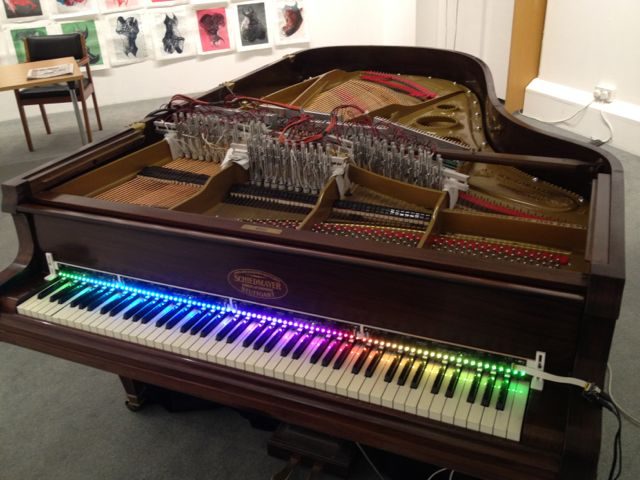
\includegraphics[width=0.99\columnwidth]{Graphics/foto/mrp-aberystwyth.jpg}
\caption[]{Magnetic Resonator Piano.\\ Electromagnetically augmented grand piano}
\label{mrp}
\end{figure}

\section{MRP (Magnetic Resonantor Piano)}

Lo strumento \emph{MRP} è un pianoforte ideato da Andrew McPherson dotato di
elettromagneti  che inducono direttamente vibrazioni nelle corde del pianoforte, generando vibrazioni acustiche indipendentemente dai martelletti, senza la
necessità di amplificazione esterna.

Si generano così \emph{sustain} infiniti, variazione di intonazione e nuovi
timbri, il tutto controllato dalla tastiera del pianoforte. L'\emph{MRP} è
stato inizialmente progettato come un'estensione del pianoforte, consentendo
al pianista di modellare continuamente ogni nota in termini di dinamica,
intonazione e timbro, pur mantenendo la ricchezza e le sfumature del pianoforte
a coda acustico.

L'\emph{MRP} è in grado di fornire sonorità diverse da quelle del pianoforte
tradizionale infatti quando i tasti vengono premuti delicatamente gli
elettromagneti producono molte delle qualità acustiche del pianoforte
escludendo la sonorità del colpo del martelletto. Utilizza 88 attuatori elettromagnetici per coprire l'intera gamma del pianoforte. Quando un singolo
magnete è attivo la relativa corda, o il gruppo di corde, di acciaio viene
tirata verso l’alto e di conseguenza quando la corrente viene interrotta la
corda ritorna nella posizione originale. Modulando la corrente alla frequenza
della corda o ad un suo armonico, la corda viene fatta vibrare senza essere mai
stata colpita dal martello. I segnali audio per gli elettromagneti provengono
infine da un computer,controllato dalle azioni dell’esecutore sulla tastiera.
È possibile un'ampia gamma dinamica che comprende anche toni appena superiori
al silenzio. Sulla tastiera del pianoforte è posizionata una barra scanner
ottica personalizzata che registra l'angolo continuo di ciascun tasto e manda
il segnale al computer\footnote{Andrew Mcpherson, \emph{The magnetic resonator
piano brings continuous note shaping to the acoustic piano}.
\url{https://instrumentslab.org/research/mrp.html}}.

\begin{figure}%[t!]
\centering
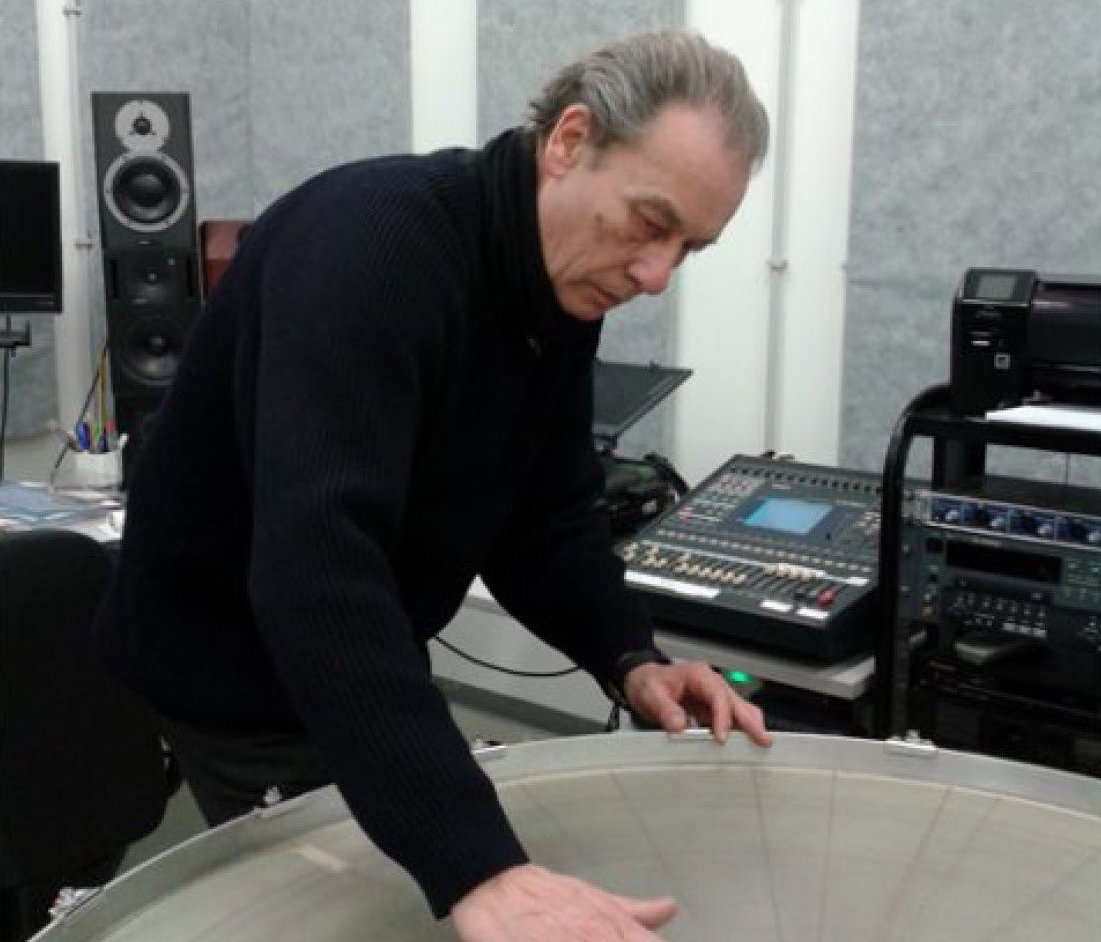
\includegraphics[width=0.99\columnwidth]{Graphics/foto/michelangelo_lupone_recadre}
\caption[]{Michelangelo Lupone.\emph{Feed-drum}.}
\label{mrp}
\end{figure}

\section{Feed-drum}

Il \emph{feed-}drum, nasce in seguito ad in lavoro musicale e scientifico
intorno all’opera \emph{Gran Cassa} (1999) di Michelangelo Lupone.

\begin{quote}
La grancassa sinfonica, lo strumento a percussione più grave, è stata introdotta
nell’orchestra solo nel XVIII secolo e nel secolo successivo ha raggiunto la
forma che oggi conosciamo.

In particolare la forma che era stretta e lunga, com’è rimasta nelle bande
militari, è stata portata a 80-90 cm di diametro e 35- 50 cm di fusto; questo
è chiuso da uno o da ambedue i lati con membrane di pelle naturale tenute in
diversi modi da sistemi che provvedono a regolarne anche la tensione.
La versione più grande, adeguata ai massimi organici orchestrali, è chiamata
grancassa imperiale, ha due membrane e raggiunge 102 cm di diametro. [\ldots]
L’utilizzo della grancassa, per quanto sostanziale in orchestra e costante da
Mozart in poi, è considerato secondario e ristretto a pochi modi di emissione
del suono: il rullo (nota lunga), spesso finalizzato al crescendo, il colpo di
riempimento 4 nelle sequenze ritmiche.

Non sono studiate tecniche specifiche, come nel caso dei timpani, e i battenti
tipici sono la mazza e le bacchette da timpano. L’idea di un’opera musicale,
interamente basata su questo strumento, è nata dall’osservazione dei modi
vibrazionali della membrana.
\end{quote}

Questo strumento fu costruito con lo scopo di studiare i comportamenti di una
membrana sottoposta a una sollecitazione impulsiva, isolando i modi armonici.

\begin{quote}
Le sperimentazioni sono state fatte con l’intento di raggiungere i seguenti
obiettivi:

\begin{enumerate}
  \item variazione della frequenza di base attraverso l’introduzione di vincoli
nodali posti sulla membrana,
  \item distinzione di più timbri in base al tipo, al modo e alla posizione
dell’eccitazione,
  \item modulazione del suono attraverso glissandi, vibrati, portamenti e
micro-articolazione ritmica,
  \item variazioni continue e a gradini della dinamica, in base al tipo di
  smorzamento imposto alla membrana.
\end{enumerate}

\end{quote}

Sulla grancassa fu applicato un microfono a contatto collegato ad un altoparlante
posizionato sotto la membrana.
L’altoparlante ha un diametro di 18 pollici ed é posizionato ad una distanza di
11 cm dalla membrana superiore.

La presenza della seconda pelle della gran cassa , oscillando a fase diverse
dalla principale, non permetteva di tenere l’intonazione della fondamentale di
$30Hz$ e per questo venne rimossa.

Inoltre il corpo con i tiranti della gran cassa fu appositamente costruito da un
artigiano in metallo per mantenere meglio l’accordatura.

Per lo stresso motivo per la membrana fu adottato  un materiale sintetico in
quanto una vera pelle sarebbe stata più soggetta a deformazioni con il tempo.
Il sistema così ideato riesce ad innescare un processo di feedback, tale da far
oscillare la membrana in modo tale che il suono ha una durata tendente
all’infinito.

L’interprete ha a disposizione un pedale di espressione con cui controlla
l’intensità del feedback.

\begin{quote}
Lo smorzamento della membrana e il conseguente decadimento del suono, si possono
regolare, così da isolare i modi alti di vibrazione con l’azione combinata dei
nodi posti sulla membrana dall’esecutore tramite le mani e della quantità di
energia immessa nel feedback. La sperimentazione del sistema ha permesso di
individuare e di segnare sulla superficie della membrana una mappa semplificata
dei modi oscillatori basata sulle fusioni di Bessel composta da 13 diametri e
8 cerchi nodali
\end{quote}

\begin{figure}%[t!]
\centering
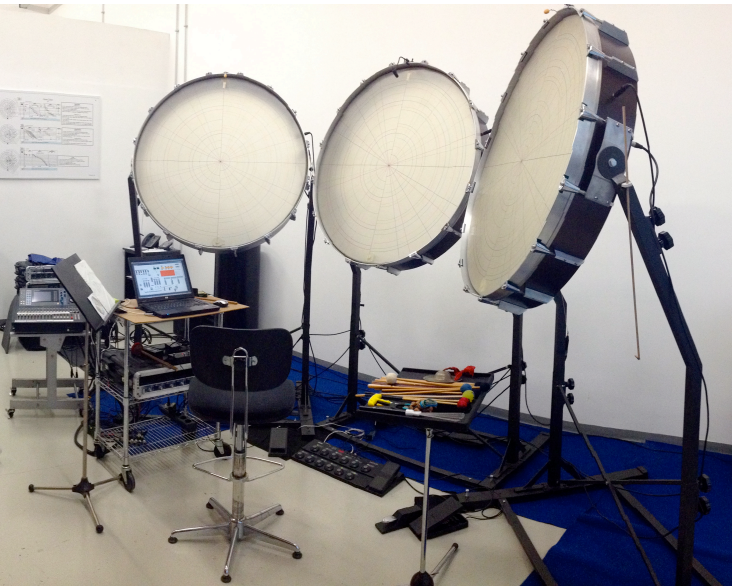
\includegraphics[width=0.99\columnwidth]{Graphics/foto/skin-act}
\caption[]{Michelangelo Lupone.\emph{Skin-Act}.}
\label{skinact}
\end{figure}

\section{Skin-Act}

In continuità con il \emph{Feed-drum}, gli \emph{Skin-Act} sono strumenti a percussione aumentati. In comune con hanno il fatto di avere una membrana di grancassa ma
mentre per il primo il feedback è generato tramite un altoparlante woofer posto
sotto la membrana, per gli \emph{Skin-Act} si ottiene tramite uno shaker applicato
sulla pelle stessa.

\begin{quote}
L’opera parte dall’idea di riprodurre lo spazio acustico, che è intorno
all’interprete, anche intorno all’ascoltatore, con caratteristiche coerenti di
mobilità e localizzazione. [\ldots]
Per realizzare una scrittura musicale che potesse evidenziare questa idea,
Lupone si è ispirato al concetto di spazio percepito e misurato attraverso il
tempo.[\ldots]

I ritmi e le durate rappresentano il materiale compositivo di base di
“Spazio curvo” sul quale vengono articolati i timbri eterogenei dello SkinAct.

L’opera è formalmente divisa in cinque sezioni, ognuna delle quali propone una
diversa concezione del ritmo:
\begin{enumerate}
  \item “nel suono” (battimenti ottenuti con le frequenze parziali della membrana),
  \item “nello spazio” (ritmi derivati dalla percezione dei movimenti e delle
localizzazioni dei suoni nello spazio acustico),
  \item“del suono” (ritmi ottenuti con tecniche di scomposizione temporale del
suono e ricomposizione a densità diverse),
  \item“con il suono” (ritmo organizzato con accenti e pause),
  \item“poliritmia” (ritmi diversi sovrapposti temporalmente).
\end{enumerate}

I tre \emph{Skin-Act} posti a distanza ravvicinata, si influenzano reciprocamente dando
luogo a una complessità elevata del fenomeno sonoro, e delle tecniche di
controllo.
\end{quote}

\begin{figure}%[t!]
\centering
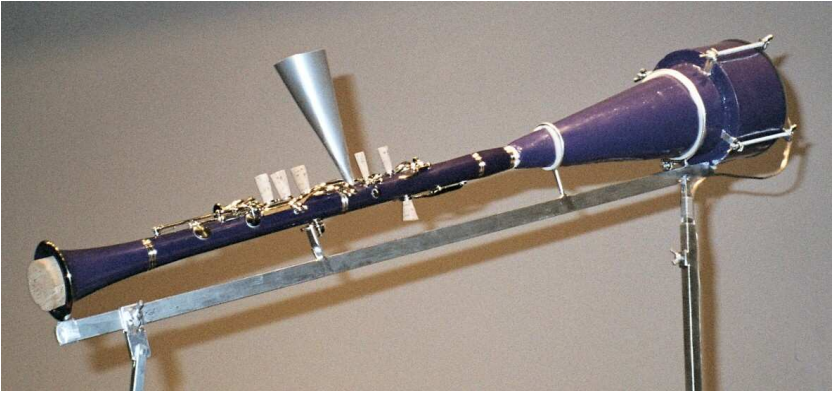
\includegraphics[width=0.99\columnwidth]{Graphics/foto/clarinetto_sospeso.PNG}
\caption[]{Silvia Lanzalone.\emph{Clarinetto Sospeso}.}
\label{clarinetto}
\end{figure}

\section{Il Clarinetto Sospeso}

Il \emph{Clarinetto Sospeso} è uno strumento aumentato costruito per il brano
\emph{Il Suono Incausato} (2005) da Silvia Lanzalone.

Questo strumento aumentato prevede l’uso del sughero con cui sono realizzati
sette tappi e tre leve: i tappi hanno lo scopo di chiudere i fori, le  leve
hanno lo scopo di tenere aperte o chiuse le chiavi. In partitura è indicato come
disporli.

Inoltre sono a disposizione dell’interprete quattro coni, uno di alluminio e tre
di cartone che vengono inseriti in determinate zone dello strumento per
amplificare l’irradiazione del suono. Completano lo strumento un cono di
piombo, scelto perché è un materiale acusticamente isolante ma non
fonoassorbente, inserito al posto del bocchino contenente un altoparlante e
un’asta di metallo su cui lo stesso strumento è fissato.

Durante l’esecuzione l’interprete è in grado di variare le sonorità emesse
dentro l’altoparlante operando manualmente om chiudendo manualmente le chiavi o
inserendo nei fori i tronchi di cono a sua disposizione.

\begin{quote}
Il \emph{Il Suono Incausato} propone una singolare installazione intorno al
clarinetto, in cui il rapporto con lo strumento non è più perseguito nella
tipica concatenazione logico-temporale per cui il suono (effetto) è ottenuto
tramite eccitazione della colonna d’aria presente nel tubo attraverso l’ancia
da parte dell’esecutore (causa). Il nuovo strumento, denominato
\emph{Clarinetto Sospeso}, è acusticamente autonomo poiché, anziché essere
“suonato” dall’interprete, viene da lui “esplorato” attraverso una serie di
interventi atti soprattutto a modificare le caratteristiche fisiche del tubo e
le combinazioni di fori aperti o chiusi, creando così nuove condizioni del
sistema vibrazionale. In questo brano il clarinetto è posto su di un sostegno
ed appare come sospeso, distante dallo strumentista, nonché fisicamente
modificato. [\ldots] Le manipolazioni effettuate sul \emph{Clarinetto Sospeso}, da
me definite “esplorazioni”, possono amplificare o attenuare alcune specifiche
risonanze, possono introdurre dei ritmi timbrici in sovrapposizione al suono di
base, possono agire per imitazione o per contrasto rispetto ad una particolare
modalità di articolazione del suono preesistente, possono non produrre alcun
effetto, coerentemente con le molteplici tipologie di connessione tra azione ed
evento. Le esplorazioni sono effettuate secondo un criterio di estemporaneità,
attraverso azioni che mettono in rilievo una componente gestuale e teatrale
dell’esecuzione.[\ldots]
Nessun suono può essere realmente \emph{Incausato} dal punto di vista fisico;
tuttavia nel \emph{Clarinetto Sospeso} i termini della relazione strumento/esecutore/suono
trovano una diversa relazione consequenziale.[…].d’arte
\end{quote}

\begin{figure}%[t!]
\centering
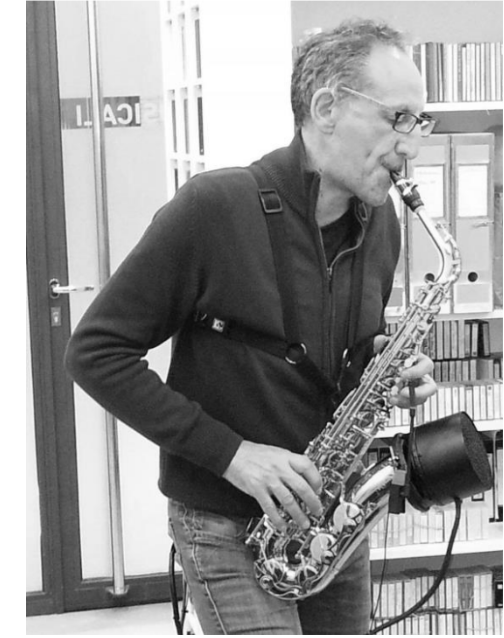
\includegraphics[width=0.99\columnwidth]{Graphics/foto/windback}
\caption[]{Enzo Filippetti.\emph{WindBack}.}
\label{windback}
\end{figure}

\section{Windback}

\emph{Windback} è uno strumento aumentato che usa il fenomeno del feedback
applicato a uno strumento a fiato.

Il primo \emph{Windback} è un prototipo ideato da Michelangelo Lupone per la sua
composizione \emph{In Sordina}. Lo strumento scelto è un sassofono a cui è stato applicato un microfono a metà del corpo e un altoparlante sulla campana.
Inoltre è contemplato anche l’uso di due pedali di controllo e un processore di
segnale.

Con questo prototipo è possibile ottenere:
\begin{enumerate}
  \item Suoni multifonici indipendenti
  \item Poliritmia
  \item Modificazione della struttura armonica
  \item Risonanza selettiva
\end{enumerate}

Questo prototipo è stato realizzato per l’opera musicale “In Sordina”.
Quest opera è stata composta utilizzando un sistema di risonanze acustiche del
sassofono caratterizzato da nuove modalità espressive.
Il flusso d’aria emesso dall’altoparlante, si propaga in senso contrario rispetto
al normale flusso d’aria prodotto da uno strumentista e genera un fenomeno di
feedback acustico in maniera potenzialmente infinita sostenendo sia la colonna
d’aria che il suono all’interno dello strumento.
Questo fenomeno permette l’esplorazione  del timbro del sassofono secondo
modalità non convenzionali e la scoperta dei dettagli del sistema di articolazione
del sassofono stesso.

\begin{figure}%[t!]
\centering
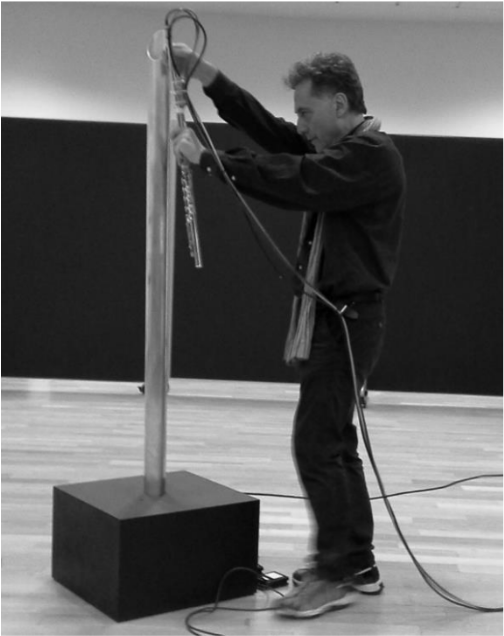
\includegraphics[width=0.99\columnwidth]{Graphics/foto/reso}
\caption[]{Gianni Trovalusci. \emph{ResoFlute}.}
\label{windback}
\end{figure}

\section{\emph{ResoFlute}}

\emph{ResoFlute} è un flauto traverso aumentato. Allo strumento tradizionale si sommano:

\begin{enumerate}
  \item due microfoni applicati internamente alla testata dello strumento al posto del
sughero tradizionale e cinque microfoni applicati esternamente.
  \item un sensore.
  \item comandi a pedale.
  \item un tubo in alluminio, di 10 cm di diametro e lungo 180 cm, per la diffusione e
la risonanza del suono.
\end{enumerate}

I cinque microfoni miniaturizzati sono fissati sul corpo dello strumento, accanto
ai fori delle chiavi, praticando dei fori nel tubo in base alla posizione di alcune chiavi. In questo modo è possibile rilevare le variazioni di pressione sonora riscontrabili nelle diverse parti del flauto.

Il corpo dello strumento è dotato di un sensore realizzato tramite una pellicola
piezo-elettrica, utilizzato per rilevare la posizione del pollice della mano
destra, che normalmente serve esclusivamente per tenere lo strumento. Un circuito
a soglia utilizza il segnale piezo-film  per produrre comandi on-off che
l'esecutore controlla in funzione della partitura.

Il suono dello strumento tradizionale è \emph{aumentato} anche attraverso l'uso
di un tubo di risonanza, che proietta il suono del flauto. Questo tubo in
alluminio è montato su di un contenitore in legno contenente un altoparlante.
L'altoparlante è collegato acusticamente al tubo attraverso un giunto conico, che aumenta l’efficacia della diffusione elettroacustica.

Tutti gli altri controlli di elaborazione del segnale vengono eseguiti tramite
pedali MIDI dotati di messaggi di variazioni di controllo e variazioni di programma.

Il flauto così \emph{aumentato} aggiunge possibilità timbriche allo strumento enfatizzando le caratteristiche di risonanza e diffusione spaziale del suono
attraverso il tubo risonante.

L'intero sistema comprende: l'algoritmo per la generazione di suoni sintetizzati
e l’elaborazione in tempo reale dei suoni del flauto. Il tutto è completato dal
fenomeno del feedback acustico.

Questo feedback dipende dalle caratteristiche del tubo risonante, responsabile
della diffusione del suono, e dalla posizione del flauto rispetto al tubo e ai microfoni interni.

L’equilibrio tra suono dello strumento ed elaborazioni elettroniche genera un
suono complesso a cui  vengono aggiunte integrazioni timbriche e diffusione
spaziale tramite la risonanza nel tubo di alluminio.

% !TEX TS-program = pdflatex
% !TEX root = ../tesi.tex

%************************************************
\chapter{Il Discreto “Astratto” e il Concreto}
\label{chp:discreto}
%************************************************

\section{La Mente Bicamerale e la Nascita del Linguaggio}

Nel testo \emph{Il crollo della mente bicamerale e l’origine della coscienza}
di Julian Jaynes si tenta di dimostrare l’affascinante teoria che la coscienza
sia una acquisizione relativamente recente (circa 1400 a.c.) dell’uomo.

Ho provato ad estrarre da questo testo alcuni concetti orientativi.

Jayenes ipotizza la possibilità che in tempi passati siano esistiti uomini  che
parlavano,giudicavano, ragionavano, risolvevano problemi, ma che non erano
affatto coscienti.

La crescita e lo sviluppo del linguaggio generò la possibilità di costruire
metafore riuscendo a passare dal concreto all’astratto: per generare concetti
astratti furono generate metafore concrete, quindi l’astratto fu generato sulle
basi della metafora.

\section{La Scrittura}

\begin{quote}
Il primo testo della storia umana che essendo scritto in una lingua che sappiamo
tradurre con sufficiente sicurezza è l’Iliade. I moderni studiosi ritengono che
questa storia  sia stata tramandata da una tradizione orale di Aedi tra il 1320
a.C.  (quando secondo indicazioni di tavolette ittite ebbero luogo i fatti
descritti) e il 900-800 a.C. quando il poema fu messo per iscritto.
\end{quote}

Jaynes spiega come gli eroi di questo poema non agiscono per scelte prese
razionalmente: in generale nell’ Iliade non esiste coscienza. Nell’Iliade  le
azioni non trovano il loro inizio in piani, ragioni e motivi coscienti, ma bensì
nelle azioni e nei discorsi degli  dei.

Chi erano questi Dei che muovevano gli uomini che obbedivano come se fossero
automi? \textbf{Erano Voci}, allucinazioni sonore: l’uomo dell’Iliade non ha soggettività,
non ha consapevolezza, non ha uno spazio mentale dove esercitare l’introspezione,
ha solo la possibilità di obbedire alle sue \emph{voci}, e in latino la parola
\emph{oboedire} è un composto di \emph{ob + audire}, udire stando di fronte a
qualcuno.

Queste allucinazioni sonore sono poi descritte come i vari dei della mitologia
greca.

Per distinguerla dalla nostra mente cosciente e soggettiva chiameremo la forma
mentale dei Micenei \emph{Mente Bicamerale}, ovvero divisa in due lobi, la
parte sinistra (\emph{cervello uomo}), logica e razionale, eseguiva ciò che
quella destra (\emph{cervello Dio}), emotiva e recettiva delle allucinazioni
sonore, le comandava.

Portando il ragionamento di Jaynes al limite, si potrebbe ipotizzare che
attualmente le pure menti bicamerali sono i nostri computer privi di coscienza,
operativi al massimo ma etero diretti dagli input dell’operatore che può essere
assimilato alla \emph{voce del Dio}.

Per molto tempo l’Iliade fu trasmessa oralmente e il mezzo utilizzato era quello
del canto e nel primo verso il cantore, l’Aedo  chiede proprio alla diva di
cantargli la storia. \emph{All’origine l’empatia era il legame di partecipazione
emotiva che univa il cantore, “l’Aedo”, al suo pubblico} Jaynes formula una teoria
nel quale anche questa diva che canta al cantore è una voce, allucinazione
sonora, che narra al cantore la successione delle vicende.

La struttura sociale di gruppi di primati dipende dalla comunicazione fra gli
individui. Quando gli individui dominanti lanciano un grido di allarme o corrono,
gli altri membri del gruppo fuggono senza nemmeno guardare quale sia la causa
del pericolo. È dunque l'esperienza di un individuo e la sua dominanza che vanno
a vantaggio dell'intero gruppo.

Non c'è ragione di pensare che l'uomo antico degli inizi del genere Homo, due
milioni di anni fa, vivesse in modo diverso.

Se il dominante  “il RE” sente una “voce”  e la rilancia  i dominati eseguono.

La mente bicamerale, con i suoi dèi che esercitavano il controllo, si evolse
come fase finale dell'evoluzione del linguaggio.

La mente bicamerale è una forma di controllo sociale ed è per la precisione
quella forma di controllo sociale che consentì all’umanità di passare dai
piccoli gruppi di cacciatori-raccoglitori alle grandi comunità agricole

Quali mutamenti permisero il passaggio dalla mente bicamerale alla coscienza?
Quando avvenne questo? Perché? Jaynes, con l’ausilio di documenti storici,
archeologici, antropologici, vede il secondo millennio a.C. come teatro di
grandi sconvolgimenti sia geografici sia culturali. L’inizio dei commerci,
l’aumento della popolazione, le guerre, misero in luce la precarietà e la
fragilità delle teocrazie bicamerali. L’avvento della scrittura, su tavolette
d’argilla, provocò l’indebolimento delle allucinazioni uditive fino all’emersione
di nuove capacità mentali, che diedero il via ad un ulteriore sviluppo della
coscienza.

Fu nel II millennio a.C., infatti, con la nascita della scrittura che si ebbe
il progressivo spegnimento dell’area destra del cervello dedicata alla ricezione
del  linguaggio emotivo (voci) e, parallelamente, la graduale prevalenza della
zona sinistra della comunicazione logico-razionale

Nella  letteratura greca, il passaggio si intravede  dalla bicamerale Iliade
alla più soggettiva  Odissea.

\begin{quote}
Il contrasto con l’Iliade è sorprendente. Tanto nelle parole quanto nei fatti e
nei personaggi L’Odissea descrive un mondo nuovo e diverso, abitato da esseri
nuovi e diversi. Gli dei bicamerali dell’Iliade, passando all’Odissea, sono
diventati deboli, si tengono sulla difensiva
\end{quote}

le azioni umane derivano dalla coscienza dei protagonisti: La grande astuzia del cavallo di Troia non è narrata nell’Iliade  ma bensì nell’Odissea e Ulisse davanti alle sirene è l’uomo che sente e vuole sentire ancora forti le “voci” bicamerali
a cui non è possibile opporsi ma la sua soggettività nascente gli suggerisce lo stratagemma fisico (le corde intorno all’albero della nave) per far si che il
suo corpo non venga trascinato dall’allucinazione verso la morte.

Il racconto biblico del Paradiso perduto può essere riletto come esemplificativo
del crollo della mente bicamerale e dell'avvento della coscienza:

\begin{quote}
Il serpente promette che $\ll$ sarete come gli elohim stessi (elohim in ebraico:
“ascolta”. È il nome in ebraico biblico della divinità e il titolo del Dio di
Israele nell'Antico Testamento), avendo la conoscenza del bene e del male$\gg$
(Genesi, 3, 5), qualità che solo l'uomo cosciente soggettivo può possedere.
E quando questi primi esseri umani ebbero mangiato dei frutti dell'albero della conoscenza, d'improvviso “ad ambedue si apersero gli occhi”, gli occhi analogali
nello spazio mentale metaforico, “ed essi si accorsero di essere ignudi” (Genesi,
3, 7), ossia ebbero una visione autoscopica e cominciarono a narratizzare,
vedendo se stessi come avrebbero potuto essere visti da altri. E così le loro
pene e i loro dolori furono “moltiplicati grandemente” (Genesi, 3, 16) e i
progenitori dell'umanità furono scacciati dal giardino dove si poteva vedere
Colui-che-è e parlare con lui come con un altro essere umano.
\end{quote}

\section{I Due Cervelli}

Da quanto scritto da Jaynes possiamo individuare la presenza nell’emisfero destro
di una potente struttura ricettiva e  sensoriale, di cui abbiamo perso la
coscienza. Alle allucinatorie  \emph{voci bicamerali} dell’emisfero destro si è
sostituito lo sviluppo della coscienza razionale  nell’emisfero sinistro. Comunque
vestigia della mente bicamerale rimangono nel mondo moderno come  l’adorazione
di statue, le apparizioni, la superstizione oltre che forme di manifesta
schizofrenia.

Federico La Sala  commentando  un  testo di Paul Watzlawick così definisce
le due metà del cervello:

\begin{quote}
Noi (come del resto altri primati) possediamo due cervelli che possono
funzionare  indipendentemente l’uno dall’altro; che non solo le due metà non
reagiscono  allo stesso modo ai medesimi stimoli  del mondo circostante, ma
che piuttosto ciascuno dei due emisferi  risponde solo a quegli
stimoli  che cadono nel suo ambito; e inoltre ogni tentativo  di influenzare uno
dei due emisferi  si deve servire della sua “lingua” specifica affinché il
segnale o la comunicazione penetrino fino ad esso. [\ldots]

L’emisfero sinistro - quello dominante nel tipico individuo destro rimane – “è
specializzato nella traduzione  della percezione del mondo circostante  in
rappresentazioni logiche, schematiche e fonetiche, e nella comunicazione  con la
realtà  sulla base di questa interpretazione del mondo in chiave logico-analitica,
Delle  sue funzioni fa parte dunque tutto ciò che è in relazione, su questa base,
con la lingua ( dunque grammatica,sintassi,semantica) e con il pensiero, e dunque
anche il leggere, lo scrivere, il contare, il fare calcoli e in generale la
comunicazione digitale”.

L’emisfero destro, invece, è altamente sviluppato per cogliere  nella loro
totalità contesti,tipi, configurazioni e strutture complesse: esso funziona
secondo il principio della “pars pro toto”, cioè  è capace di
riconoscere-ricostruire “una totalità” a partire da un dettaglio essenziale.
[\ldots]
\end{quote}

In  conclusione, dell’emisfero destro è propria la “lingua analogica”,
dell’emisfero sinistro  è propria la “lingua digitale.

\begin{quote}
Il fatto dell’esistenza di queste due lingue  fa supporre che ad esse debbano
corrispondere due immagini del mondo totalmente differenti, giacché è noto  che
un linguaggio non rispecchia la realtà, ma piuttosto crea una realtà.[\ldots] É
parimenti importante  per il mio argomento la costatazione che il linguaggio
dell’emisfero destro è arcaico e non sviluppato.

Nelle scimmie la dominanza emisferica  può essere influenzata tramite rinforzi.
[\ldots]Poiché anche nell’uomo nella prima infanzia le due metà del cervello sono
ancora ampiamente indifferenziate, si può supporre che, simili rinforzi, in
grado di portare alla dominanza finale [dell’emisfero sinistro n.d.r.], siano
possibili anche dall’interrelazione fra genitori e bambino.
\end{quote}

\section{Il Senso Perduto dell’Ascolto}

Non solo l’interrelazione tra genitori e bambino determina  la prevalenza
dell’emisfero sinistro ma, come segnala  Giorgio Netti, in una lezione per
Avidi Lumi su  il ciclo dell'assedio, è il più generale processo di
“culturalizzazione” a determinare   la perdita delle sensibilità emotive
dell’emisfero destro o per dirla con Netti delle “necessità”:

\begin{quote}
La musica contemporanea corrisponde di più alle nostre necessità. Io ho
lavorato tanti anni con i bambini e mi ricordo  che facevo degli esperimenti
con i bambini: facevo sentire un Lieder di  Schubert e i bambini  ridevano,
facevo sentire un Lieder di Webern  e stavano attenti. È strano questo fatto, ma
come?È orecchiabile! Ma è bellissimo Schubert eh! Ma il nostro è un ascolto
acculturato, e quindi apprezziamo quella bellezza attraverso tutto un passaggio
di trasformazioni “colte”. Quello di Webern arriva più direttamente a quella che
è la necessità  attuale. [\ldots]
\end{quote}

Forse è proprio  la perduta coscienza di questa potente struttura ricettiva e
sensoriale dell’emisfero destro  a renderci non « immediata » la comprensione
del concetto di « intero »  descritto da Walter Branchi:

\begin{quote}
Se non si comprende il senso profondo del concetto di «Intero», dell’indiviso ,dell’eterno del tutto, non si può comprendere una musica,[\ldots] «L’intero»
non accetta l’idea di un inizio, di una fine e di una trasformazione poiché
tutto è sempre stato, quindi è senza tempo… non concepisce un’evoluzione
attraverso la tecnica o la scienza. Non porta a domande sull’origine di questo
o di quello, ma soltanto a «condividere»… non concepisce una realtà da
interpretare attraverso simboli o rappresentazioni, ma ci dispone e ci offre
l’opportunità di esistere  in tutte le cose senza nessuna guida, religione o
dottrina, [\ldots]ma semplicemente facendosi «essere» e scoprire noi stessi
come sue espressioni, risuonando con esso: « questa è la sua forza ».
\end{quote}

Se la verbalizzazione appartiene all’emisfero sinistro, il non verbalizzabile
probabilmente è un processo che  si sviluppa nell’emisfero destro. Lo sviluppo
logico-scritturale avvenuto  nell’emisfero sinistro ha sicuramente influenzato
nell’emisfero destro il complesso rapporto  tra  voce parlante ed ascolto.

Massimo Cacciari in \emph{Silenzio ed ascolto nella musica di Luigi Nono}
analizzando  il rapporto tra scrittura, voce ed ascolto,  afferma che noi
tendiamo a dare per scontato il significato culturale dell’adozione della
scrittura alfabetica che fissa  le cellule fonetiche della nostra voce,
rappresentandole visivamente. L’invenzione di un sistema di scrittura  nel
2500 a.C. circa, è una classificazione teorica, per certi versi astratta, che
verrà poi usata da tutte le culture che si svilupperanno nel bacino mediterraneo:

\begin{quote}
Prima di questa rivoluzione per comprendersi occorreva ascoltarsi, [\ldots] con
l’invenzione della scrittura alfabetica avviene una progressiva desomatizzazione
della voce, una perdita dell’udire : l’udire non è più una funzione essenziale
del comprendersi. [\ldots].Si può comprendere qualcosa semplicemente vedendo, [\ldots]
questo è il prodotto di una colossale rivoluzione culturale[\ldots]che conduce ad un
primato della scrittura  ed ad un primato della visione nell’ambito delle nostre
culture. [\ldots]..Nella lingua greca la radice del vedere è la stessa del verbo
sapere, [\ldots] vedere, leggere, sapere è la triade dominante nelle nostre culture.
[\ldots] Quindi il passaggio dal « logos » che originariamente è proprio « il dire »,
«il comunicare », «l’emettere suoni » [\ldots] al « logos » essenzialmente come testo
scritto e fissato. [\ldots]Il problema di un dominio della visione, di un dominio della
scrittura, [\ldots] di una perdita di un rapporto con la voce e con il parlare [\ldots]
[è il problema] con cui si scontra gran parte della musica contemporanea più
avvertita culturalmente. [\ldots]. Il dominio prepotente del congelamento
discorsivo-concettuale del significato, la perdita del rapporto vivo con la
parola viva, [\ldots] è un problema che non può essere dimenticato dalla musica.
Perché la musica non può essere senza ascolto,e quindi la perdita della
dimensione dell’ascolto[\ldots] è fatale per la musica. [\ldots]
\end{quote}

Le esperienze musicali più avvertite culturalmente  del ‘900 si interrogano
intorno a questo suo presupposto:

\begin{quote}
Ma c’è chi ascolta ? In questa nostra
cultura dominata dal vedere [\ldots] vi può essere chi ascolta ?Infatti la
musica, sotto un certo spetto, si fa sempre più semplice, la musica di consumo
evita di misurarsi  con il problema del rapporto con la voce parlante, anche
con l’aleatorietà della voce parlante[\ldots].
Se io ritengo che la mia prassi musicale  si esaurisca nella definizione di una
sequenza fonetica e che questa sia consegnata ad un testo scritto, ecco che la
musica diventa esattamente come qualunque altro discorso, ed presuppongo che il
rapporto con quella musica sia scontato allorché io l’ho scritto, [\ldots] si presume
che quella musica scritta verrà ripetuta sempre eguale. [\ldots] Ma questo non è
accettare la morte dell’ascolto? E se accetto la morte dell’ascolto[\ldots]decreto
una sorta di suicidio della musica. [\ldots].
\end{quote}

Le esperienze musicali più avvertite culturalmente  del ‘900 vogliono,

\begin{quote}
in modo provocatorio, costringere all’ascolto, non ammettono distrazioni,
[\ldots] la difficoltà fondamentale di questo tipo di musica [\ldots] è che
costringe ad un ascolto non distratto, cioè ci costringe a ricordare che
questo organo, « l’ascolto » noi probabilmente lo abbiamo perduto.
\end{quote}

Giorgio Netti sintetizza 3 differenti modalità d’ascolto chiamandole ascolto
predatore, ascolto analitico e ascolto sospeso:

\begin{quote}
L’ascolto predatore tende a
focalizzarsi sull’eventuale presenza di oggetti sonori evidenti e inusitati
(siano questi figure, nuove tecniche strumentali, usi differenti di tecniche
conosciute o l’insieme dei tre), per estrarli dal contesto e usarli, allo stato
solido irrigiditi nel loro essere a questo punto identificati come oggetti. [\ldots]

L’ascolto analitico è un ascolto a strati, si allunga su archi più estesi
mettendo in relazione gli aggregati fra loro, isola via via alcuni elementi a
suo avviso portanti che (come le campate di un ponte) gli servono da appoggio
alla tenuta dell’attenzione sull’intera durata.

Questo ascolto più degli altri si può tradurre in segno musicale, grafico,
matematico, verbale, e proprio per questa sua alta conducibilità/traducibilità
è diventato lo strumento degli innumerevoli studi che affollano lo spazio
musica. Solo apparentemente oggettivo, è molto influenzato dalla gerarchia di
valori precedentemente stabilita[\ldots]

Se l’ascolto analitico procede per campate, l’ascolto sospeso (non interrotto,
sospeso) è l’azzardo di una campata lunga fino al termine del passaggio nella
sua intera durata: è l’ascolto più aperto perché presuppone la capacità di
sospendere momentaneamente le categorie interpretative che abitualmente ci
caratterizzano; riuscire a farlo vuol dire riuscire ad ascoltare ciò che ci è
proposto in sè e non in relazione a noi (in relazione a quello che noi pensiamo
sia interessante, giusto, storicamente fondato, etc). [\ldots]
\end{quote}

\section{L’Astratto nel Linguaggio, nella Musica e nella Rappresentazione Visiva}

Il dominio della visione sull’ascolto come classificazione ideale e razionale,
citato da Cacciari, è un concetto assolutamente parallelo  al crollo della mente
bicamerale e l’origine della coscienza  di Jaymes , ambedue conseguenti
all’invenzione della scrittura alfabetica, Possiamo dedurre che l’acquisizione
della coscienza e  l’invenzione  scrittura conseguente allo sviluppo del
linguaggio, hanno  rappresentato l’evolversi   di un processo logico e razionale
del lobo sinistro esautorando e sostituendo  il ruolo direzionale dell’emisfero
destro emotivo e ricettivo.

Per poter generare concetti astratti fu necessario  generare metafore ed
analogie, che sono il frutto di un ragionamento logico e razionale. La logica e
la razionalità hanno accompagnato, seguendo il ragionamento di Cacciari, il
passaggio dal « logos » che originariamente è proprio « il dire »,
«il comunicare », «l’emettere suoni » al « logos » essenzialmente come testo
scritto e fissato. Parallelamente questo processo investe il concetto che la
prassi musicale  possa esaurirsi nella definizione di una sequenza fonetica e
che questa sia consegnata ad un testo scritto : la notazione e lo spartito.

Una tale prassi musicale  si rispecchia nel concetto di ascolto analitico di
Giorgio Netti, nella sua alta traducibilità in segno musicale, grafico,
ùmatematico e verbale, solo apparentemente oggettivo.

Possiamo dedurre quindi che, in generale,  l’acquisizione della coscienza ha
determinato una rappresentazione semplificata della realtà, per dirla con Netti,
solo apparentemente oggettiva, che potremmo definire « astratta » in quanto
generata da schemi logici. Tale astrattizzazione  ha la grande qualità di essere
facilmente comunicabile e trasmissibile,  ma ha il grande difetto di non
comprendere ciò che è stato represso  da questo processo nell’emisfero  destro:
la coscienza della presenza   di una potente struttura ricettiva e  sensoriale
studiata da Jaynes, l’organo « ascolto » citato da  Cacciari, l’ascolto « sospeso »
nella definizione di Netti.

Si può notare come una parallela « razionalizzazione »  si è prodotta nella
storia della rappresentazione visiva  nel rapporto tra visione retinica
« naturale » e proiettata su una superficie concava e rappresentazione
prospettica « artificiale » proiettata su un piano. Fu Leon Battista Alberti,
architetto e umanista ( 1404-1472) nel trattato “De Pictura” (1435-1436,
stampato nel 1511) ha definire  le regole della "costruzione legittima"
(cioè della proiezione centrale con punto di distanza),e ad a suddividere la
prospettiva in:

\begin{itemize}
  \item prospettiva come metodi di rappresentazione\\
  \item “perspectiva naturalis” o “communis”, ossia la scienza della visione
  \item “perspectiva artificialis” o “pingendi”, ossia la scienza della rappresentazione
\end{itemize}

\begin{quote}
La costruzione prospettica esatta astrae radicalmente dalla struttura dello
spazio fisiologico : non solo il risultato ma anche il suo fine è [quello] [\ldots]
di trasformare lo spazio psico-fisiologico in quello matematico, [\ldots]e se tra i
nostri contemporanei soltanto pochissimi hanno riconosciuto quelle curvature ciò
dipende senza dubbio, o almeno in parte,dall’abitudine ( confermata anche
dall’osservazione della fotografia) alla costruzione prospettica piana.
\end{quote}

Successivamente alla fotografia l’abitudine alla costruzione prospettica centrale
è stata progressivamente amplificata  dalla fruizione del cinema, prima, e
della televisione poi, infatti tutti questi sistemi visivi sono basati, sia in
ripresa che in visione, sulla proiezione dello spazio circostante su di una
superficie piana. La diffusione ed il tempo di fruizione dei personal computer
ha ulteriormente contribuito all’assuefazione di questa modalità « astratta »
della rappresentazione del circostante.

Quindi se la nostra epoca,

\begin{quote}
la cui visione era condizionata da una
rappresentazione dello spazio che si esprimeva attraverso una rigorosa
prospettiva piana ,doveva riscoprire le curvature del nostro mondo visivo, per
così dire, sferoide, queste curvature erano invece del tutto ovvie per un’epoca
abituata si a vedere  secondo la prospettiva, ma non la prospettiva piana: cioè
per l’Antichità classica.
\end{quote}

Infatti Vitruvio nel quarto capitolo del terzo libro  del suo trattato
\emph{I dieci libri dell’architettura} trattando delle fondamenta dei templi
scrive:

\begin{quote}
se invece si deve erigere un podio su tre lati della costruzione, bisogna far si che i
plinti, le basi, i fusti, le cornici e le cimase si fondano armonicamente con
lo stilobate che si trova alla base delle colonne. Esso dovrà essere livellato
in modo che, per effetto degli scamilli impari, presenti nel mezzo un
rigonfiamento, altrimenti darebbe l’impressione di essere concavo.
\end{quote}

Significativo al riguardo anche un passo del Decameron  scritto da Giovanni
Boccaccio nel XIV  secolo, prima quindi della codificazione albertiana della
prospettiva centrale,in cui nella quinta novella della sesta giornata, così
viene descritto Giotto:

\begin{quote}
ebbe uno ingegno di tanta eccellenza, che niuna cosa dá
la natura, madre di tutte le cose ed operatrice col continuo girar de’ cieli,
che egli con lo stile e con la penna o col pennello non dipignesse sí simile a
quella, che non simile, anzi piú tosto dessa paresse, intanto che molte volte
nelle cose da lui fatte si truova che il visivo senso degli uomini vi prese
errore, quello credendo esser vero che era dipinto.
\end{quote}

Quindi non solo per l’Antichità classica, per dirla con Panofsky, ma ancora nel
XIV secolo  Boccaccio vedeva la pittura di Giotto, più vera del vero, e tale
pittura non era certo caratterizzata dall’adozione della prospettiva centrale
teorizzata circa un secolo dopo dall’Alberti.

Abbiamo analizzato tre canali di comunicazione : il linguaggio, la musica e la
rappresentazione  spaziale.

In tutti questi canali abbiamo  riscontrato la prevalenza dello svilupparsi,
anche se in tempi diversi , di una progressiva tendenza verso l’astratto  per
facilitare la comunicazione.

Schematizzando possiamo dire che la scrittura, la notazione e la
rappresentazione prospettica centrale,  sono stati dei processi che
incasellando le infinite emotività  in schemi logici, geometrici e fissati
all’interno delle proprie regole razionali, hanno reso « astratto » nel lobo
sinistro  ciò che  pervadeva, senza regole  e assiomi , in modo « concreto »
il lobo destro.

Potremmo stabilire un collegamento tra questo ragionamento e  quanto scrive
Schaeffer  a proposito del concetto di «concreto»:

\begin{quote}
Noi abbiamo chiamatola nostra musica « concreta », poiché essa è costituita da elementi preesistenti, presi in prestito da un qualsiasi materiale sonoro sia rumore  che musica
tradizionale. Questi elementi sono poi composti in modo sperimentale mediante
una costruzione diretta  che tende a realizzare una volontà  di composizione
senza l’aiuto, divenuto impossibile di una notazione tradizionale.
\end{quote}

Quindi riassumendo, con la prevalenza della logica  il linguaggio,
schematizzandosi in un « astratto», è diventato scritturale. La riproducibilità
della scrittura per lungo tempo è stata affidata alla manualità dei copisti,
tale riproducibilità si è enormemente allargata con l’invenzione della stampa
per quasi  universalizzarsi con l’avvento del computer e dell’era digitale.

Un percorso confrontabile lo ha intrapreso la rappresentazione grafica con la
schematizzazione logico-geometrica della prospettiva centrale « astratta ».
Tale rappresentazione  del circostante è rimasta inalterata con l’avvento della
fotografia in cui il rapporto obiettivo-pellicola piana risulta identico alla
costruzione geometrica della prospettiva centrale. La diffusione  del cinema,
prima, e della televisione, poi, dello stesso metodo di rappresentazione
spaziale  ha contribuito sempre più all’assuefazione  del nostro sistema
percettivo  a questa modalità rappresentativa. Di nuovo l’era digitale e
l’adozione del computer, vagliando un numero enorme di immagini sul piccolo
schermo, hanno consolidato l’assuefazione a questo modo « astratto » di
percezione visiva.

Anche la musica con il progressivo sviluppo tecnico degli strumenti musicali e
con la progressiva definizione  del sistema di notazione si è fatta via via
sempre più « astratta » in quanto trascrivibile in partitura  e « discreta ».
« Discreta » perché nell’infinità delle frequenze è stata scelta una logica
matematica, il sistema temperato, basato sulla   radice dodicesima di due.  La
notazione e la successiva diffusione a stampa degli spartiti, come la scrittura
e la rappresentazione prospettica, hanno  contribuito alla diffusione ed
all’assuefazione  a questo sistema « astratto ».

Il problematico rapporto  tra compositore e partitura nella musica contemporanea
del 1960 è così descritto da Massimiliano Mila nel \emph{La linea Nono (A proposito
de Il canto sospeso)}:

\begin{quote}
[\ldots] Può darsi benissimo che al compositore, oggi, per esprimersi in maniera
valida sia necessario riconoscere ed attuare le leggi intrinseche che governano
la struttura della materia sonora. Purché, appunto, al travaglio di questo
volontario assoggettamento al determinismo della materia si riconosca una
funzione meramente strumentale: di lì oggi si deve passare perché la musica
continui a vivere quale è sempre stata, come una manifestazione dell’uomo, e
naturalmente dell’uomo di oggi, manifestazione dotata di autenticità specifica e
di originalità, non tale che si limiti a ripetere le esperienze precedenti
ormai cristallizzate in formule convenzionali.

Invece la realizzazione delle leggi che governano la struttura del materiale
sonoro ha spesso l’aria di volersi porre come fine a se stessa, e pretende di
esaurire per intero la natura stessa e i fini della musica, di una «nuova musica»
che sarebbe sostanzialmente diversa, per una brusca frattura, da quella svoltasi
fino a ieri. Come se oggi, nella composizione musicale, non ci fosse più posto
per l’iniziativa dell’uomo. Come se la musica dovesse restringersi ad essere
niente più che il prodotto necessario, quasi la secrezione chimica, d’una
deterministica struttura della materia sonora. Non resta al compositore altra
libertà che quella di scegliere il punto di partenza, di stabilire le premesse
del gioco: in seguito si tratta solo di non sbagliare le operazioni e di
verificare alla fine, con un «come dovevasi dimostrare », la validità delle
regole e la loro corretta applicazione.

Se si riduce la musica a questo, allora la parte lasciata all’invenzione del
compositore è talmente insignificante, che facilmente può imporsi la tentazione
dialettica di farne sacrificio sull’altare della piena oggettivazione e
spersonalizzazione della materia sonora. L’onnipotenza di quest’ultima viene
tanto più esaltata, se l’uomo rinuncia a predisporne i dati iniziali e lascia
che essa celebri da sola i propri trionfi, proclamando in tutta la sua
lapalissiana evidenza la legge dell’identità, e rivelando al mondo attonito e
stupefatto la gran novella che a è uguale ad a.

I cervelli elettronici danno risposte pertinenti ed eseguono lavori utili
all’uomo, perché l’uomo ci mette dentro, in un certo ordine, dei cartellini
perforati. Lasciamo che i cervelli elettronici forino e dispongano da sé i
propri cartellini: continueranno a svolgere operazioni corrette, fornite d’una
loro interiore coerenza e perfettamente obbedienti a un sistema di leggi
numeriche. Operazioni che all’uomo non servono più, se non per una mistica
contemplazione della Legge nella sua perfezione. Tra la musica che si esaurisce
interamente nella determinazione totale e la musica vera c’è la stessa
differenza che c’è tra la riuscita di un «solitario», e tutta quella calda
lotta di astuzie tra uomini, di rischi calcolati, di assaggi esplorativi, di
botte e di parate, che è una partita a scopone.[\ldots]
\end{quote}

Per quanto riguarda la musica, in particolare, la registrazione meccanica e le
possibilità diffusive della registrazione elettroacustica ( dal vinile al nastro
magnetico) hanno definitivamente consolidato questo sistema di ascolto.
Anche in questo campo l’era digitale e l’adozione del computer hanno
definitivamente ingessato lo schema logico-matematico e quindi «astratto della
musica».

\begin{figure}%[t!]
\centering
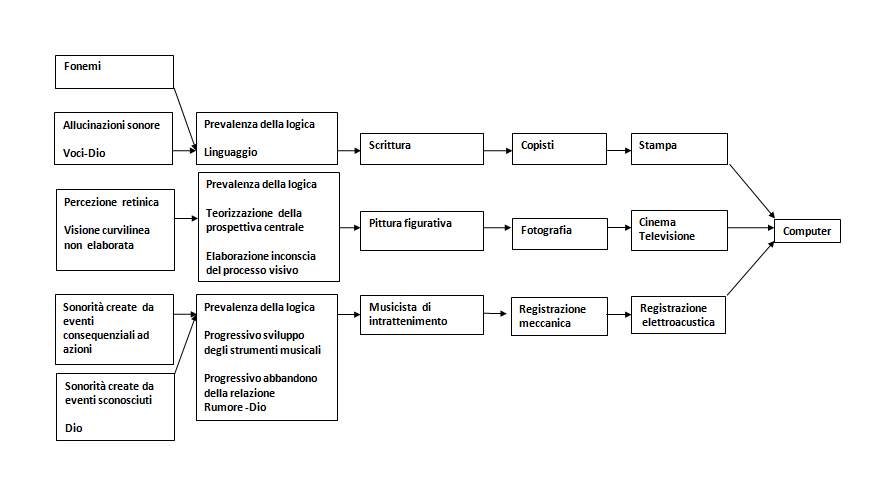
\includegraphics[width=0.99\columnwidth]{Graphics/foto/scheda_nuova}
\caption[]{}
\label{scheda}
\end{figure}

% !TEX TS-program = pdflatex
% !TEX root = ../tesi.tex

%************************************************
\chapter{NASCITA DI UN PROTOTIPO}
\label{chp:nascita}
%************************************************

Possiamo ipotizzare, quindi , il computer come una mente bicamerale : un’entità
dotata di una spropositata  capacità logico-matematica, sicuramente superiore a
quella umana, che necessita, però, di un’altra entità che gli fornisca
dall’esterno  gli input necessari ad avviare il suo percorso  standardizzato
basato su una logica  «semplicemente» binaria: questa entità esterna è l’uomo.
Per dirla con Jaynes gli uomini possono  rappresentare  gli “dei” del computer:
la silenziosa “allucinazione sonora”  che guida e indirizza la “coscienza” digitale.

Storicamente si riscontra questo tipo di sequenza: lo strumento suona, il
computer elabora e  il suono elaborato viene diffuso dagli altoparlanti.

In questo modo però, il suono elaborato perde tutte le caratteristiche di
diffusione spaziale tipiche dello strumento acustico originale, in quanto
un altoparlante dispone di una sola direzione di diffusione del suono,.

Possiamo definire questa sequenza  un processo generato  nell’area
logico-matematica “geometrica” governata dall’emisfero sinistro.

L’idea generatrice di questo studio, invertendo inizialmente la sequenza
tradizionale, è quella di far diventare l’elaborazione L.E. “l’allucinazione
sonora”, il suono nascosto, che pervade un ipotetico “emisfero destro” dello
strumento acustico, in questo caso un flauto. È all’interno di questo emisfero,
dove sono racchiusi tutti i suoni non suonabili direttamente dalle chiavi dello
strumento, che si è concentrata la ricerca, esplorando nuovi timbri e  nuove
sonorità, uscendo così dai canoni classici dello strumento.

In tal modo è stato possibile sia restituire al suono elaborato, che dare  ai
suoni sintetici, le stesse caratteristiche di diffusione del suono acustico
facendo risuonare l’elaborazione L.E. dentro lo strumento.

Di conseguenza  viene annullato il divario spaziale tra suono L.E. e suono
acustico, essendo il flauto l’unica sorgente emissiva di suono.

Questo modo di diffusione potrà avere sia la funzione di generatrice di
sonorità, ma potrà anche essere usata parallelamente alla sequenza tradizionale,
in modo tale da non avere una sola direzione ma due che hanno come uscita
finale solamente lo strumento acustico.

Questo tipo di struttura sonora  permette di pensare il ”dispositivo” così
assemblato come   un unico strumento  che necessita della contemporanea
collaborazione di due persone: lo strumento in questo modo diventa un luogo di
incontro e collaborazione tra i due interpreti per la ricerca di nuove timbriche.

Come strumento da aumentare è stato scelto un flauto per due motivi: si voleva
lavorare sul flusso d’aria e il flauto è uno strumento a fiato non dotato di ancia.

Per realizzare questo  sistema era necessario immettere nel flauto un flusso di
onde di pressione generato dal live electronics.

Prima di giungere al dispositivo che ha restituito il risultato attualmente più
efficace sono stati elaborati una serie di prototipi.

Il primo passo è stato quello di analizzare un flauto studiandole sue
caratteristiche sia di emissione che strutturali.

Questa analisi si è concentrata soprattutto sulla testata del flauto in quanto l’onda prodotta doveva precedere l’imboccatura.
Tra l’imboccatura e la parte posteriore del flauto, chiusa da una ghiera, è collocato un tappo di sughero rimovibile. Questa è stata la zona su cui si è deciso di intervenire.

\begin{figure}
\centering
\subfloat[]
{
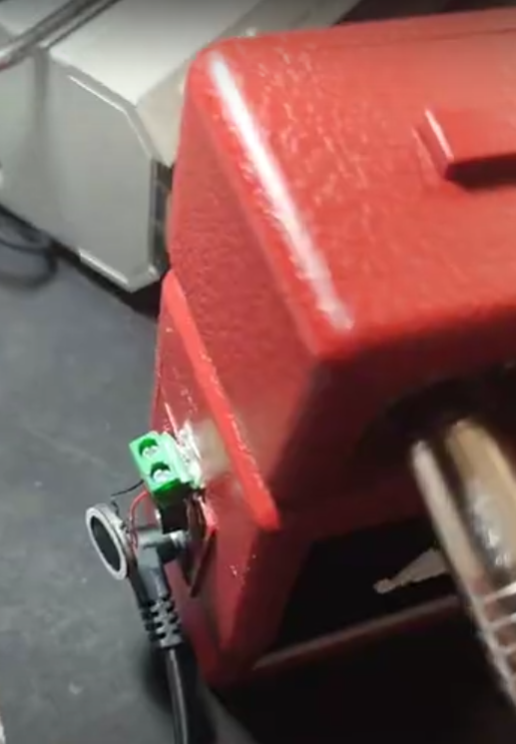
\includegraphics[width=.45\columnwidth]{Graphics/foto/alto.PNG}} \quad
\subfloat[]
{
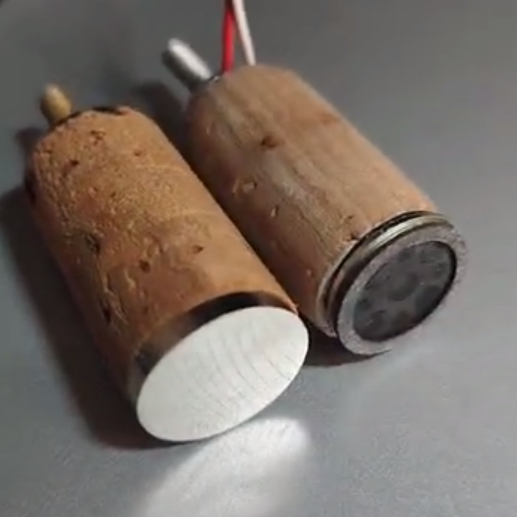
\includegraphics[width=.45\columnwidth]{Graphics/foto/tappo_parlante.PNG}}
\caption{Tappo Parlante}
\end{figure}

\section{Il tappo-parlante}

La prima idea è stato quello di convertire proprio il tappo di sughero in un altoparlante. Presa la misura del diametro interno del flauto, 18mm,si è cercato se nel mercato esistevano altoparlanti da 17mm. L’ altoparlante di questo diametro è di 1watt e 8 ohm. Per farlo suonare è stato usato un mini amplificatore per chitarra Marshall a cui era collegato di fabbrica  un altoparlante di diametro maggiore ma con le stesse caratteristiche. Tale altoparlante è stato scollegato ed è stato collegato il mini altoparlante di 17mm, con risultati sonori accettabili.

Il tappo da flauto è caratterizzato da un foro interno che permette il passaggio di una piccola asta filettata, dotata di testata di blocco, necessaria alla sua regolazione tramite la ghiera finale.
La prima idea è stata quella di forare il tappo  parallelamente al foro originario per far passare i cavi dell’altoparlante.
La parte del tappo verso l’imboccatura è stata scavata internamente in modo da poter consentire sia l’arretramento della testa della asta filettata, sia l’inserimento del mini altoparlante.
Per fare ciò è stato necessario sostituire l’asta filettata originale con una vite che avesse una testa di diametro inferiore al diametro del tappo. In questo momento sembrava ancora necessario mantenere la possibilità di regolazione dell’altezza del tappo all’interno della testata del flauto.
Logicamente questo progetto ha comportato la necessita di forare la ghiera di regolazione in due punti per far passare i cavi.

Nella foto è possibile vedere il confronto tra un tappo originale della testata di un flauto e d il tappo elaborato per questo prototipo.

La fisionomia dell’altoparlante è stato il problema di questo prototipo.
Infatti il suono di questo altoparlante non è prodotto tramite l’oscillazione di un corpo ma bensì dalla messa in vibrazione di cristalli. Tale vibrazione non è in grado di  produrre uno spostamento d’aria dentro la canna del flauto anche a causa del ridottissimo diametro dell’altoparlante. Oltretutto il suono prodotto dall’altoparlante era completamente dal suono del flautista ed essendo così piccolo l’altoparlante aveva una risposta che non contemplava minimamente le basse frequenze.

\begin{figure}
\centering
{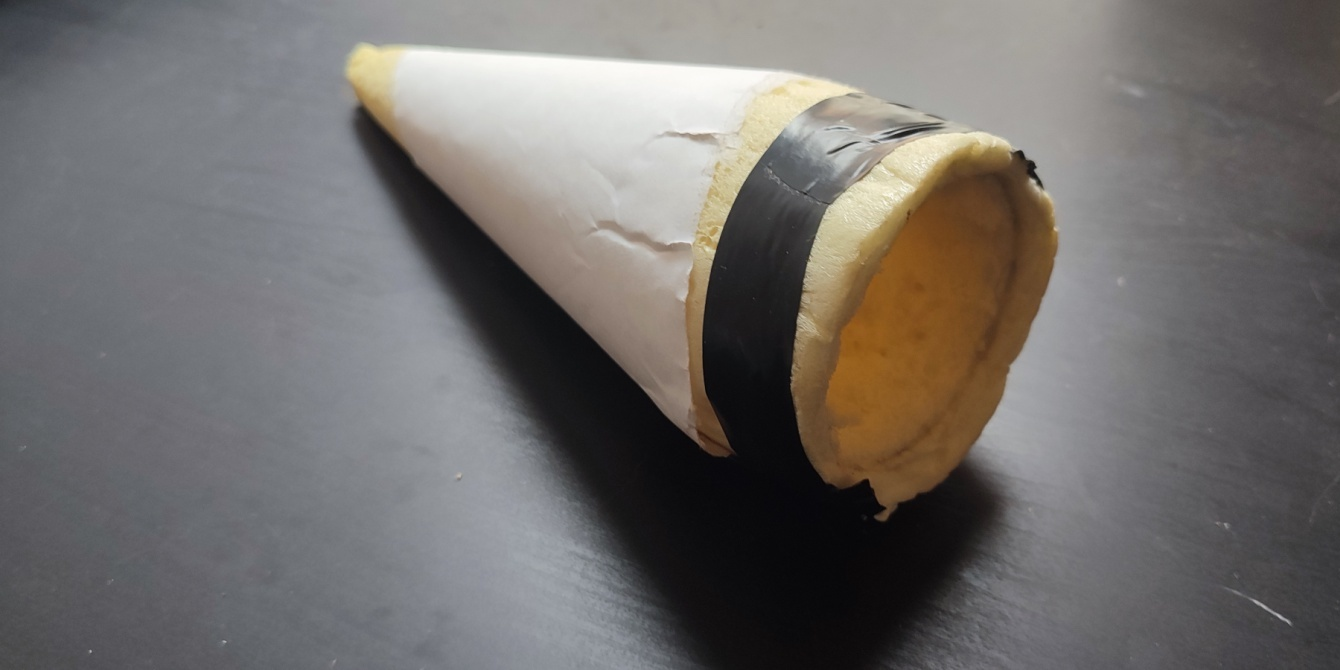
\includegraphics[width=.98\columnwidth]{Graphics/foto/schiuma}}
\caption{Cono di Schiuma}
\label{fig:schiuma}
\end{figure}

\section{Il cono di schiuma}

Dopo il fallimento del tappo-parlante è stato necessario cambiare l’approccio  progetto.

In un flauto l’elemento principale che genera suono è la colonna d’aria in movimento. Questa colonna d’aria, cambiando diteggiatura, cambia lunghezza e di conseguenza cambia l’intonazione.
Era necessario, quindi, per mettere in movimento la colonna d’aria del flauto un altoparlante di dimensioni notevolmente superiori a quelle del tappo-parlante.
Il primo tentativo di convogliare un flusso d’aria dentro il flauto fu realizzato tramite un cono di schiuma espansa, internamente cavo, collegato da una parte con un altoparlante di 7cm di diametro e dall’altra con la testata del flauto a cui era stato tolto il tappo interno. Logicamente l’altoparlante era collegato ad un amplificatore a cui arrivavano segnali generati da un computer.

Il problema principale di questo prototipo era soprattutto l’instabilità del sistema creata da peso dal peso dell’altoparlante. Parallelamente nacque il

proposito di poter sfruttare dia la parte positiva che negativa della vibrazione della membrana dell’altoparlante.



\section{Il primo imbuto}

\begin{figure}
\centering
\subfloat[]
{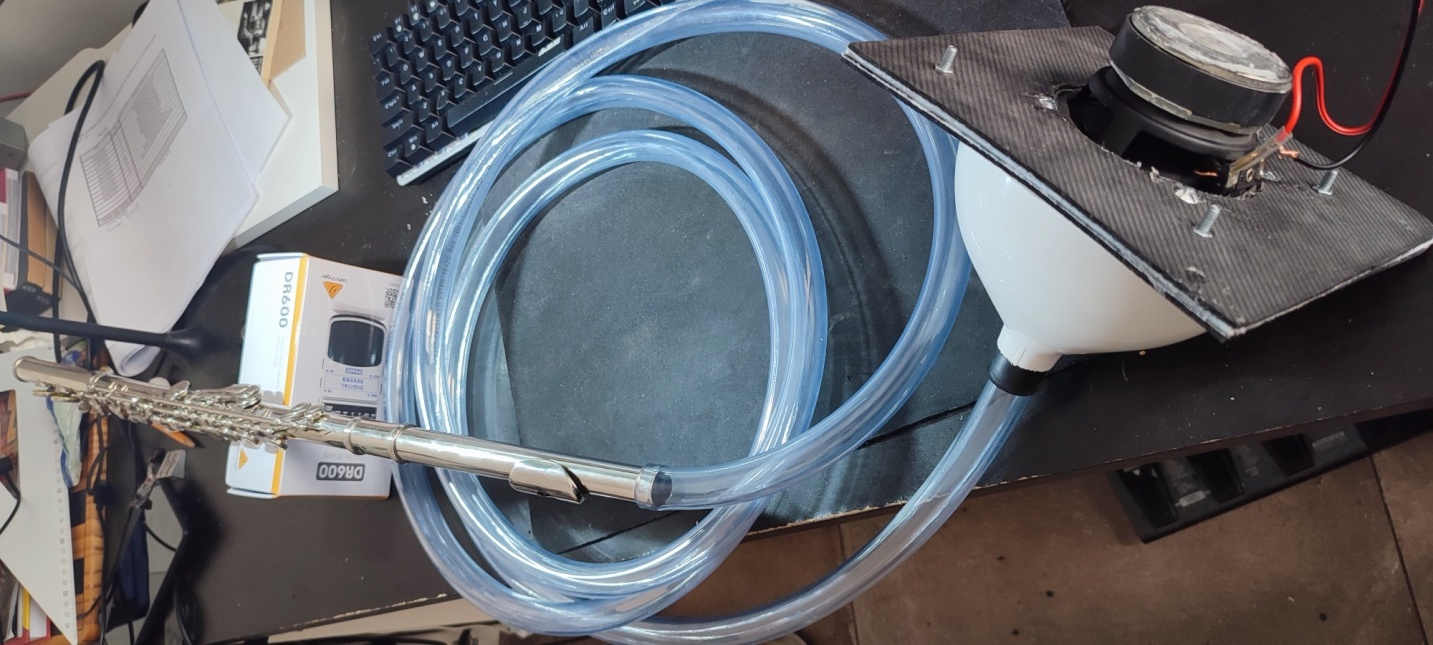
\includegraphics[width=.99\columnwidth]{Graphics/foto/imbuto1}} \\
\subfloat[]
{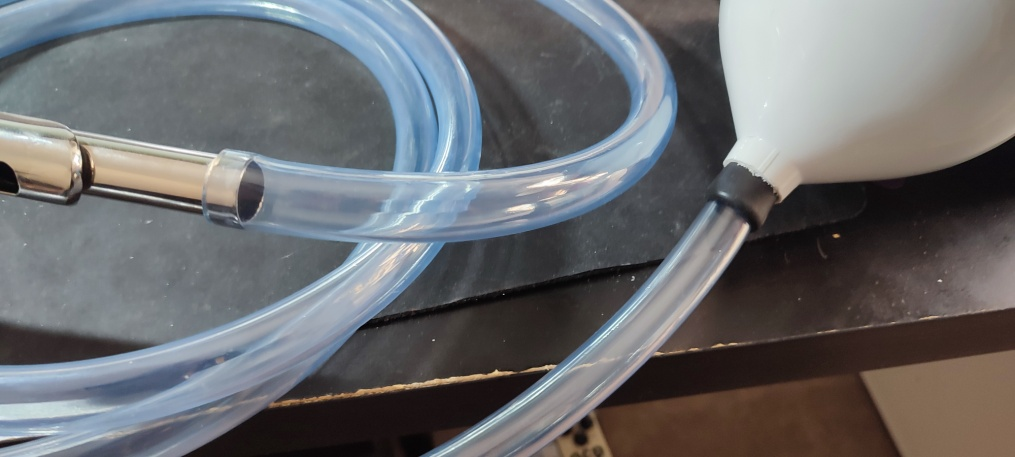
\includegraphics[width=.99\columnwidth]{Graphics/foto/imbuto2}}
\end{figure}

Vista la fragilità strutturale del cono di spugna si è pensato di sostituire il
collegamento tra l’altoparlante e il flauto con un imbuto collegato al flauto tramite un tubo di gomma.  Il collegamento tra l’imbuto e il tubo è stato
realizzato tramite un gommino antiscivolo per sedie forato, in grado di compensare la differenza di diametro tra il foro dell’imbuto e il tubo di gomma.

Per questo prototipo è stato scelto un tubo di gomma con il dimetro interno identico al diametro esterno del flauto in modo da poter realizzare un incastro.
Per raccordare l’altoparlante all’imbuto è stata usata una lastra di plexiglass rivestita da entrambi i lati due tappetini per il mouse forati con funzione di guarnizione. Inizialmente si è pensato di posizionare l’altoparlante da un

lato della lastra e l’imbuto dall’altra. Successivamente, come da foto, sia l’altoparlante che l’imbuto sono stati montati dallo stesso lato della lastra.
Il flusso all’interno del flauto, però, risultava ancora debole per cui si è pensato di sfruttare sia la fase positiva che quella negativa della membrana dell’altoparlante.

\begin{figure}%[t!]
\centering
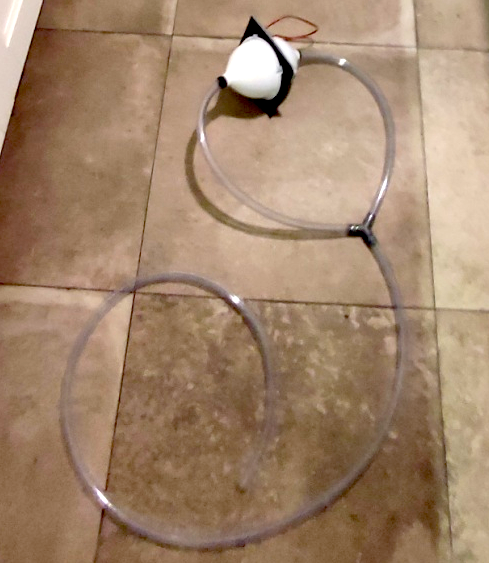
\includegraphics[width=0.99\columnwidth]{Graphics/foto/biconico}
%\caption[]{Magnetic Resonator Piano.\\ Electromagnetically augmented grand piano}
%\label{mrp}
\end{figure}

\section{Il Biconico}

Vista la presenza delle guarnizioni sulle due facciate della lastra si è pensato di montare un secondo imbuto identico al precedente sul retro l’altoparlante.

I due tubi convergono a metà percorso in un unico tubo, che si collega alla testata del flauto, tramite un raccordo Y.
Il flusso derivante da questo nuovo tentativo risultò ancora insufficiente ad innescare la colonna d, aria all’interno del flauto.

Tale mancanza di flusso venne imputata alla dimensione ridotta dell’altoparlante e quindi venne progettato un sistema identico con un altoparlante di 5 pollici di diametro.
Inoltre i due imbuti non erano sufficienti  schermare verso l’esterno le sonorità generate dall’altoparlante.

\begin{figure}[ht!]
\centering
\subfloat[]
{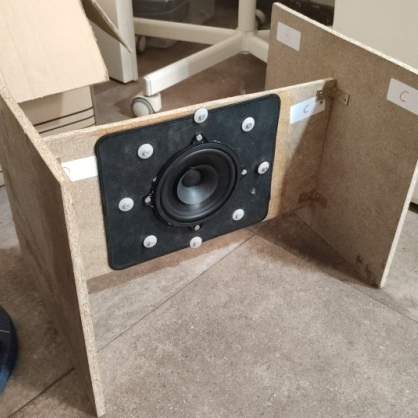
\includegraphics[width=.45\columnwidth]{Graphics/foto/scatola1}} \quad
\subfloat[]
{\label{fig:example-b}%
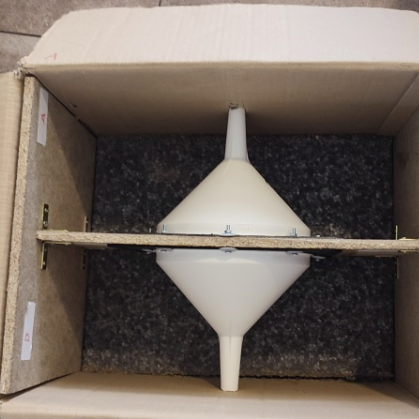
\includegraphics[width=.45\columnwidth]{Graphics/foto/scatola2}} \\
\subfloat[]
{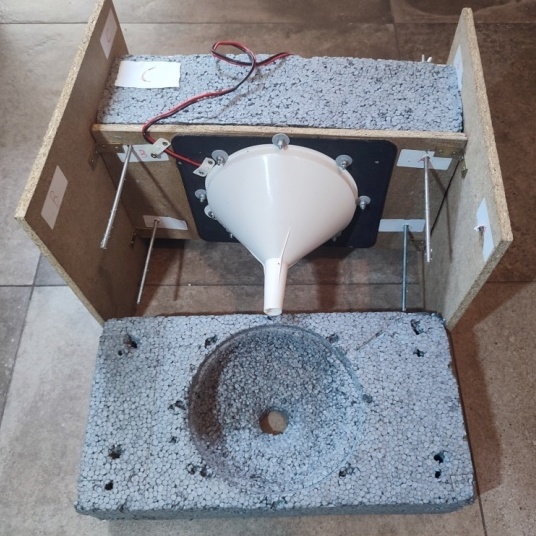
\includegraphics[width=.45\columnwidth]{Graphics/foto/scatola3}} \quad
\subfloat[]
{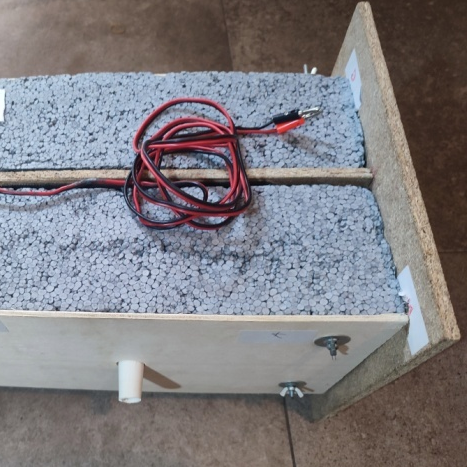
\includegraphics[width=.45\columnwidth]{Graphics/foto/scatola4}}
\caption{Scatola per il biconico}
\label{fig:scatola}
\end{figure}

\section{La Scatola}

Con lo stesso procedimento l’altoparlante da cinque pollici e due nuovi  imbuti di diametro adeguato sono stati montati su una lastra di legno.
Con la previsione di dover insonorizzare quanto prodotto dall’altoparlante  si è pensato ad un supporto a forma di H in grado di poter essere inserito in una scatola di cartone il cui fondo era foderato di polistirolo [Fig. \ref{fig:scatola}].

Il rettangolo di polistirolo è stato sagomato in modo tale da permettere l’inserimento dei supporti verticali tra la parete della scatola e la stessa tavoletta di polistirolo.

Per l’insonorizzazione dei due imbuti si è provveduto a scavare  all’interno di una tavola di polistirolo  un volume simile al negativo dell’imbuto.
Per ricavare una sagoma adatta è stato foderato un imbuto con un foglio di carta vetrata  a grana grossa  in modo tale che pressando e ruotando  questo imbuto sul polistirolo si è scavata la relativa sagoma [Fig. \ref{fig:scatola}].


Per l’applicazione dei pannelli di polistirolo laterali alla struttura ad H, si è fatto ricorso a quattro barre filettate passanti  e due  tavolette di legno.  Le tavolette di legno sono state applicate mediante dei dadi a farfalla  in modo da far aderire la tavolette sul polistirolo e di conseguenza sugli imbuti [Fig. \ref{fig:scatola}].

L’insonorizzazione si è completata inserendo un coperchio di polistirolo con al centro delle sagomature per farlo coincidere con la parte superiore della struttura ad H.

Si è ipotizzato che la mancanza di un elevato flusso all’interno del flauto dipendesse dalla scarsa velocità del flusso stesso determinata dalla  sezione del tubo di gomma usato. È stato necessario, quindi, progettare un raccordo in grado di collegare il diametro del foro dell’imbuto con il ridotto diametro del nuovo tubo. Nuovamente sono stati usati i gommini antiscivolo per sedie.

È stato possibile infatti inserire nella parete del gommino l’elemento in plastica di uno stop a cui era stata tagliata la  parte finale. Questo è stato possibile in quanto il diametro esterno  della parte in plastica dello stop si adattava perfettamente ai 7mm del diametro interno del nuovo tubo. Un tubo di diametro ridotto ha permesso di entrare direttamente nella testata del flauto e collegarsi al tappo tramite l’inserimento all’interno del tappo stesso  di una identica parte in plastica di stop [Fig. \ref{fig:scatola}].

\begin{figure}[t!]
\centering
\subfloat[]
{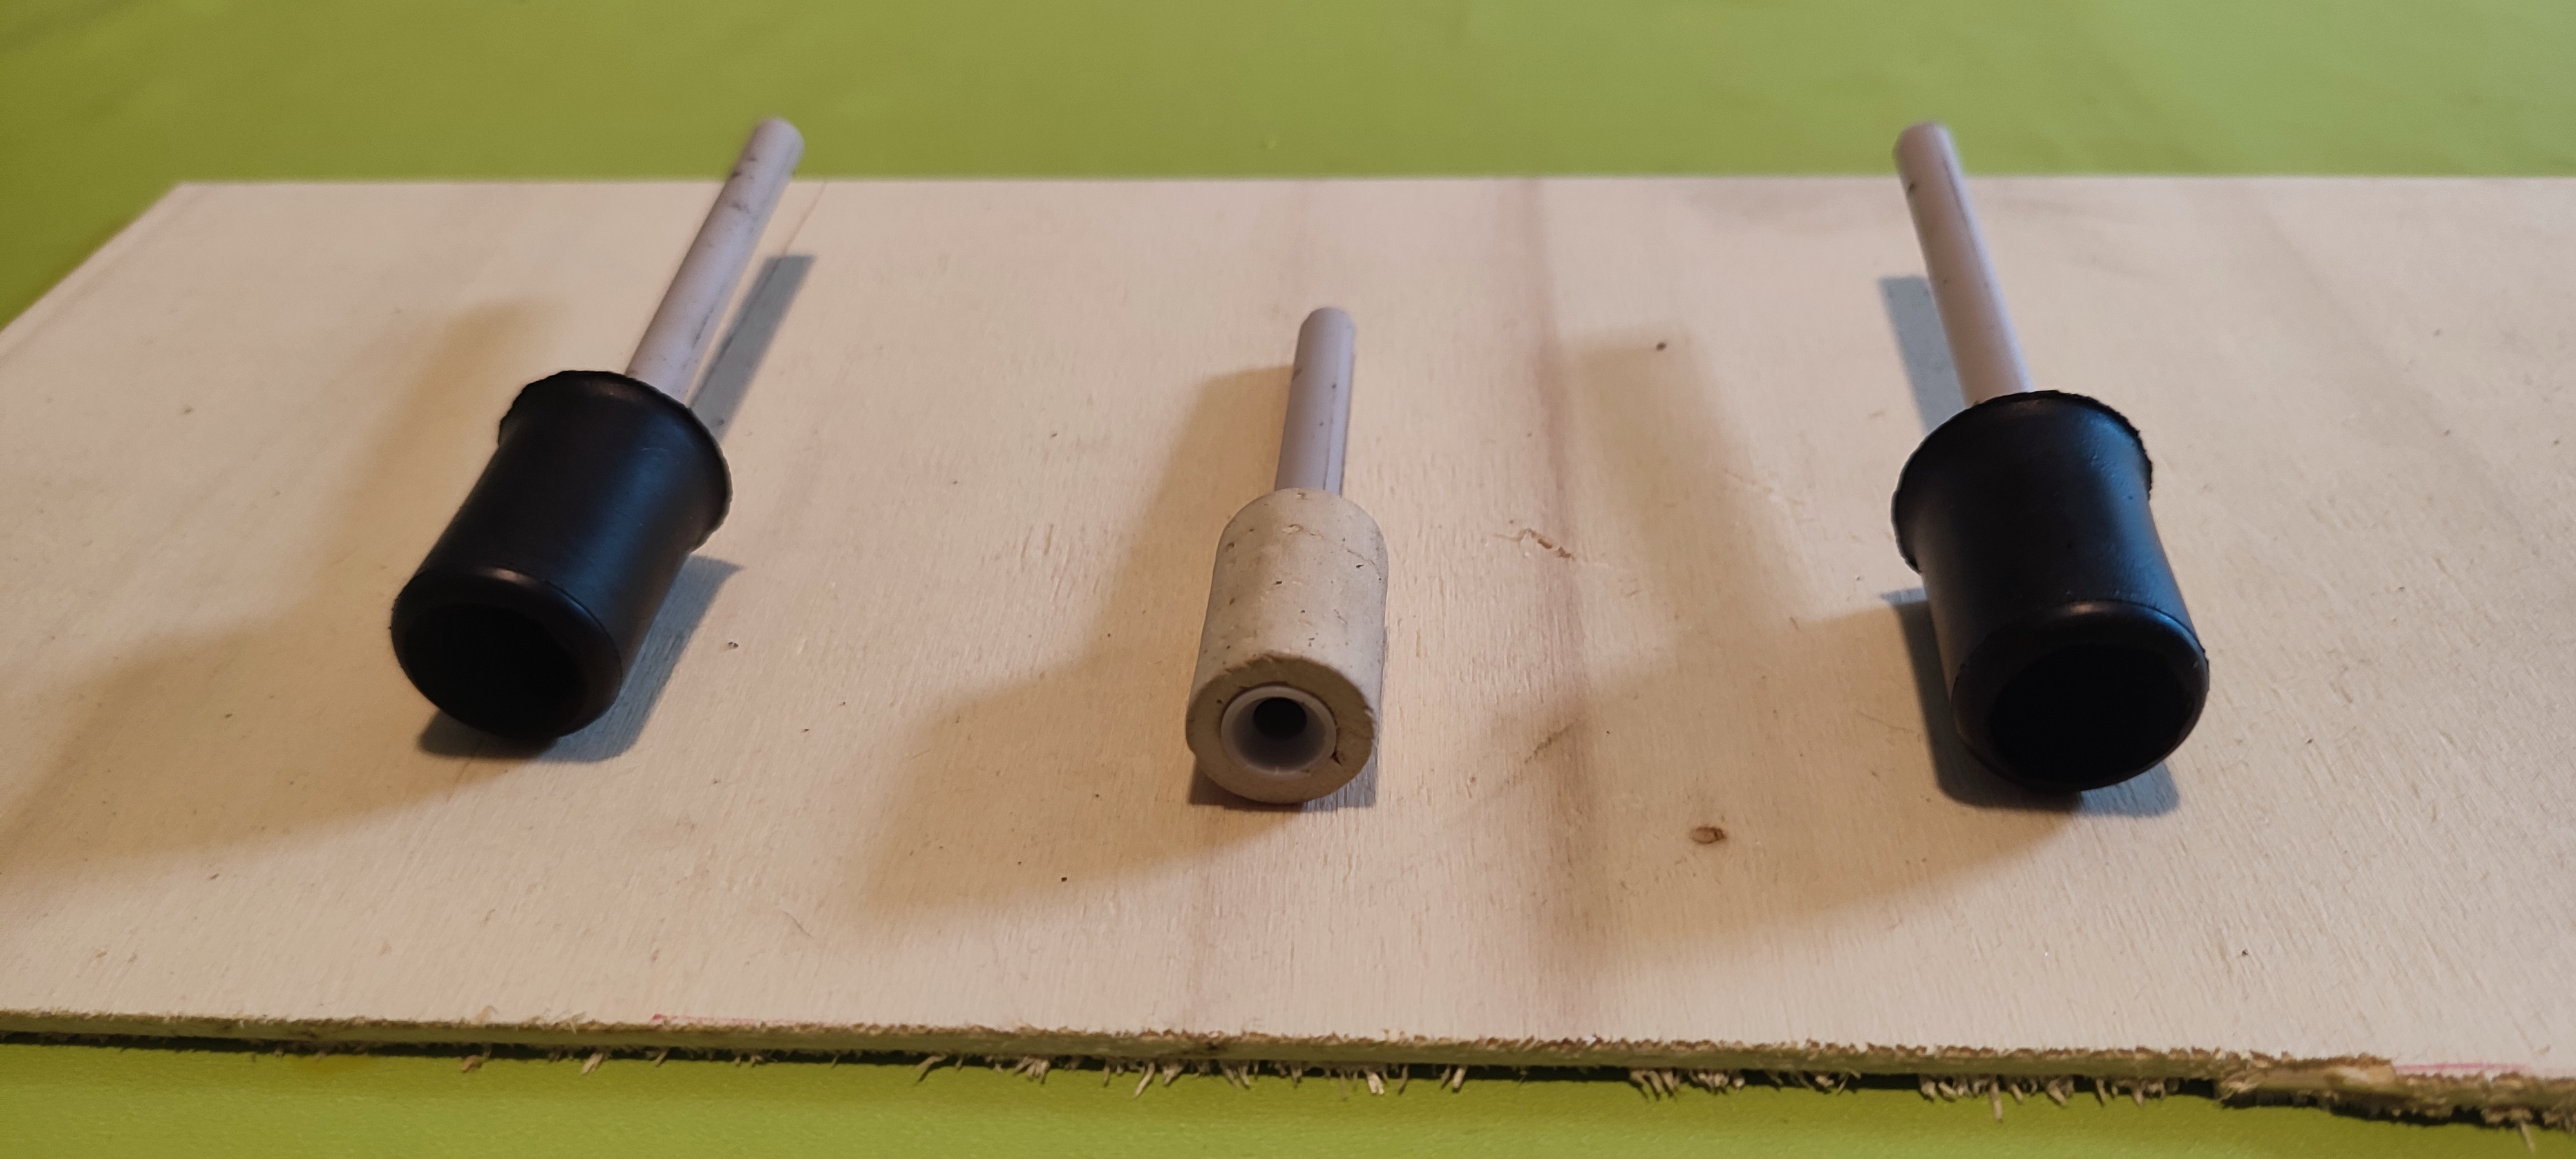
\includegraphics[width=.99\columnwidth]{Graphics/foto/1694686916414}} \\
\subfloat[]
{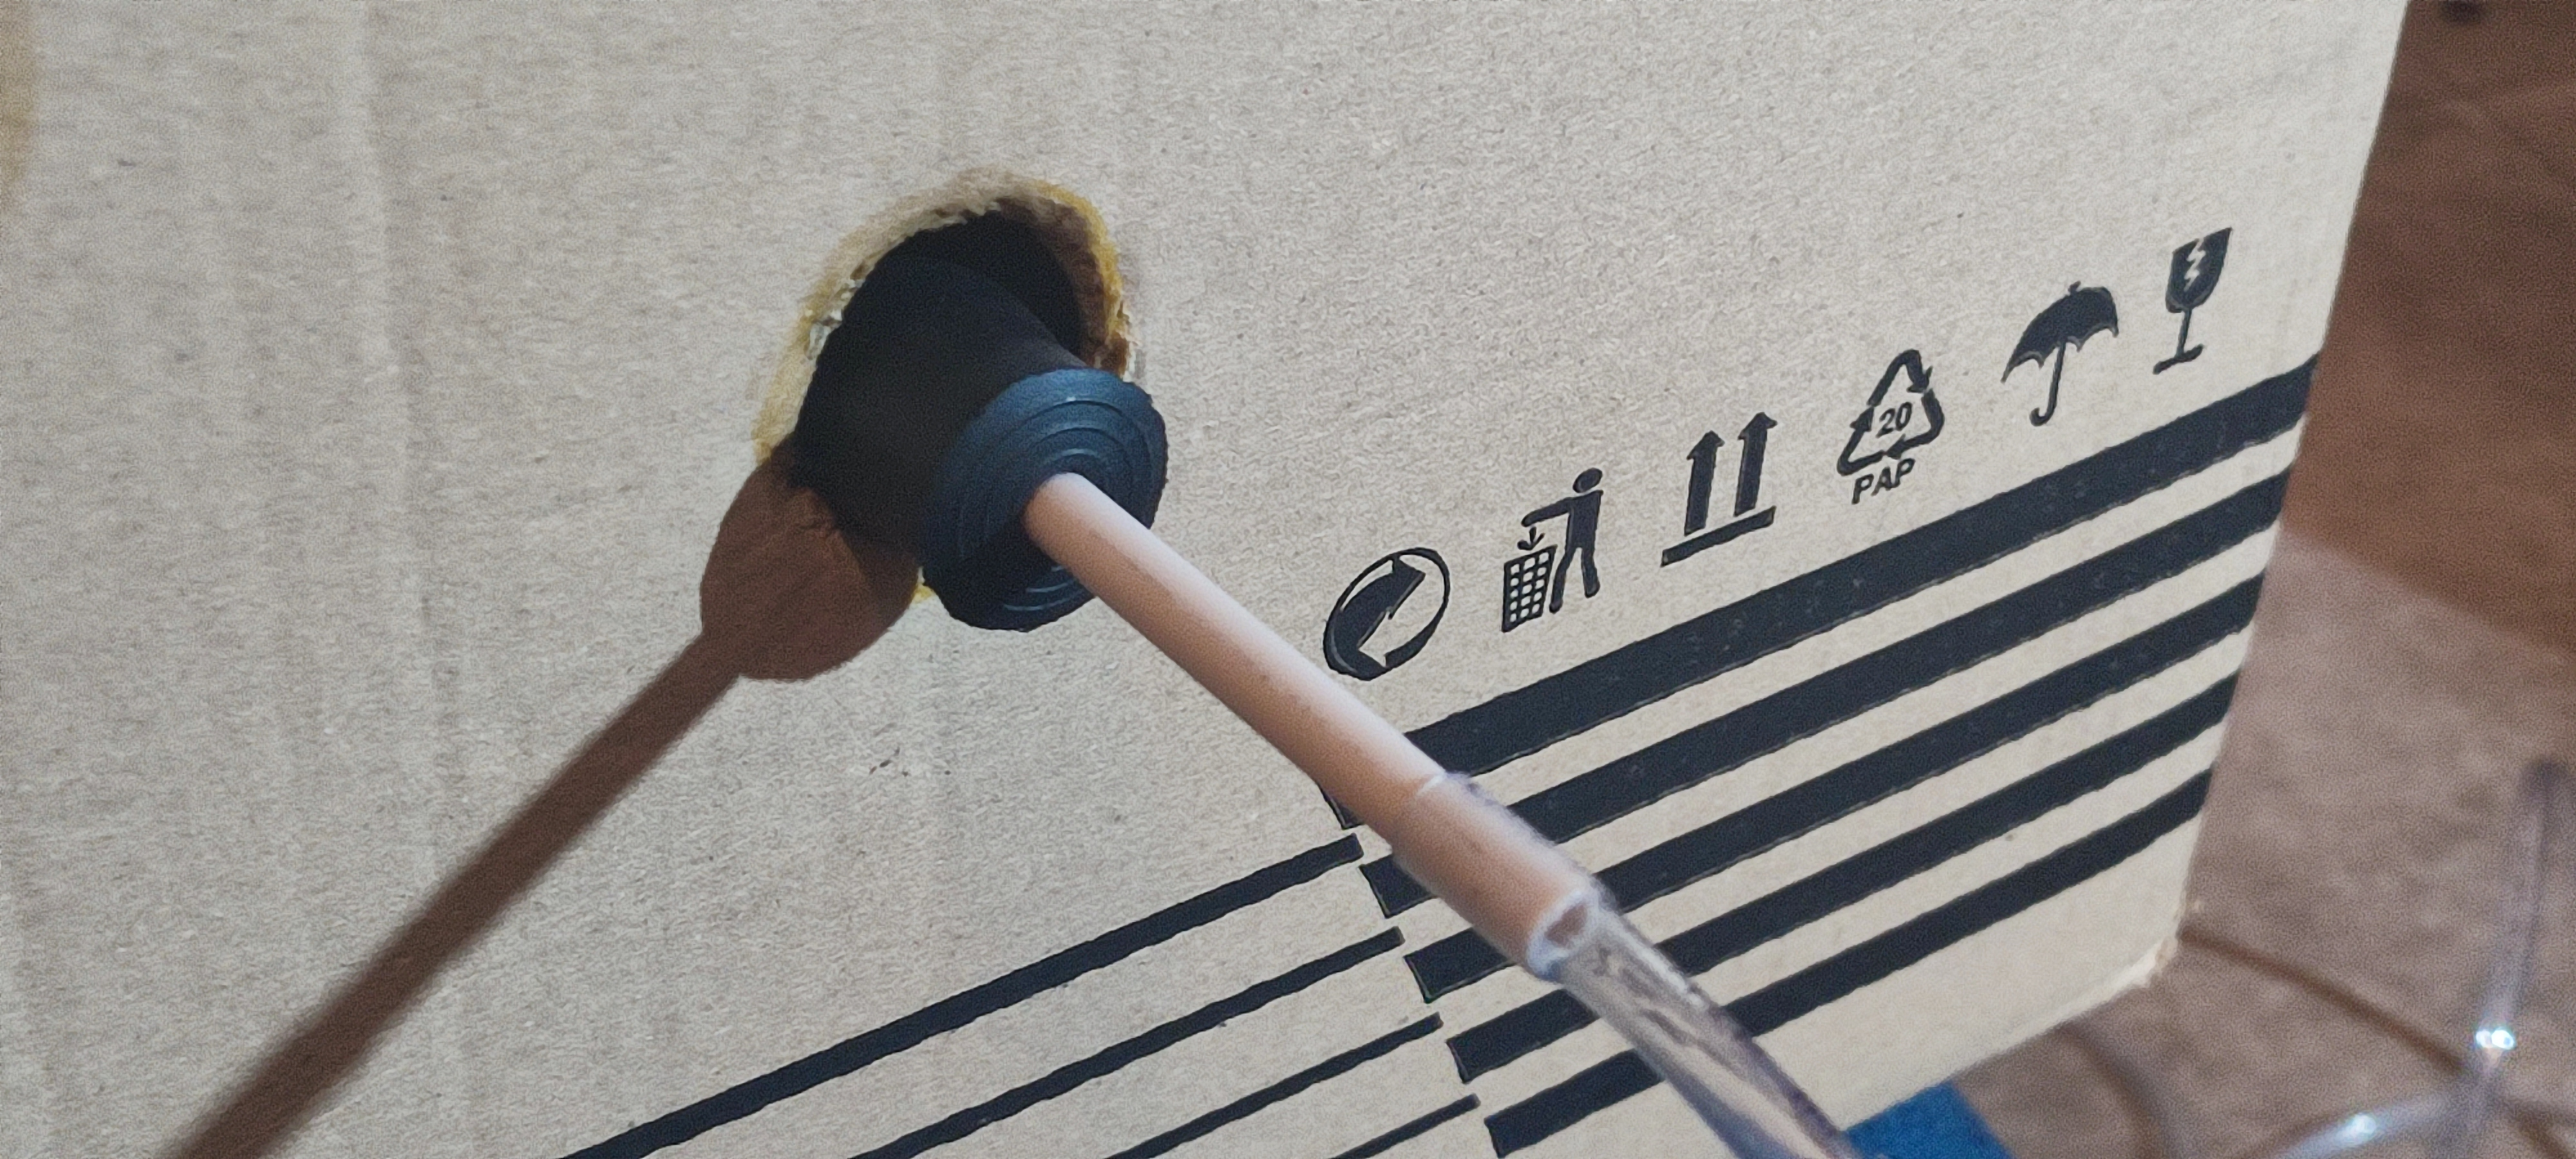
\includegraphics[width=.99\columnwidth]{Graphics/foto/1697469349089}}
\caption{Riduttori di pressione}
\label{fig:example}
\end{figure}

I due tubi collegati agli imbuti si collegano al tubo che entra dentro al flauto con un collegamento a $Y$ simile al precedente “biconico” ma di diametro ridotto.

Rendendo operativo questo muovo sistema (collegamento computer, amplificatore, altoparlante, flauto) nuovamente venne riscontrato uno scarso flusso all’interno del flauto. Tale mancanza di flusso era determinata da due fattori:

\begin{enumerate}
  \item Il doppio flusso teorizzato in realtà tendeva a zero in quanto il flusso positivo generato dello spostamento della membrana era annullato dal contemporaneo spostamento negativo della membrane stessa.
  \item L’effetto desiderato all’interno del tubo del flauto non dipendeva dalla         velocità del flusso determinata dalla ristretta sezione del tubo di gomma ma dalla pressione dell’aria all’interno del tubo stesso.
\end{enumerate}

Da queste considerazioni si è deciso sia di utilizzare solo la parte positiva dello spostamento della membrana dell’altoparlante che di aumentare il diametro del tubo di gomma in modo da accrescere la pressione del flusso.
Queste scelte consentivano tecnicamente di poter usare un altoparlante più grande in modo da sfruttare il più possibile l’aumentata pressione del flusso.

\section{Il Flauto Bicamerale}

Per generare un flusso adeguato è stato adottato un altoparlante subwoofer da 8 pollici, diametro esterno di $21 cm$, con una potenza di $300 Watt$ e con un’impedenza di $4 \Omega$:

Come contenitore è stato scelto un imbutone per lo smaltimento dei calcinacci in pvc composto da un cilindro attaccato a un tronco di cono.
Il diametro del cilindro è di $21,7 cm$ di poco superiore ai $21 cm$ del diametro esterno dell’altoparlante [Fig. \ref{fig:imbutone}].

\begin{figure}
\centering
\subfloat[]
{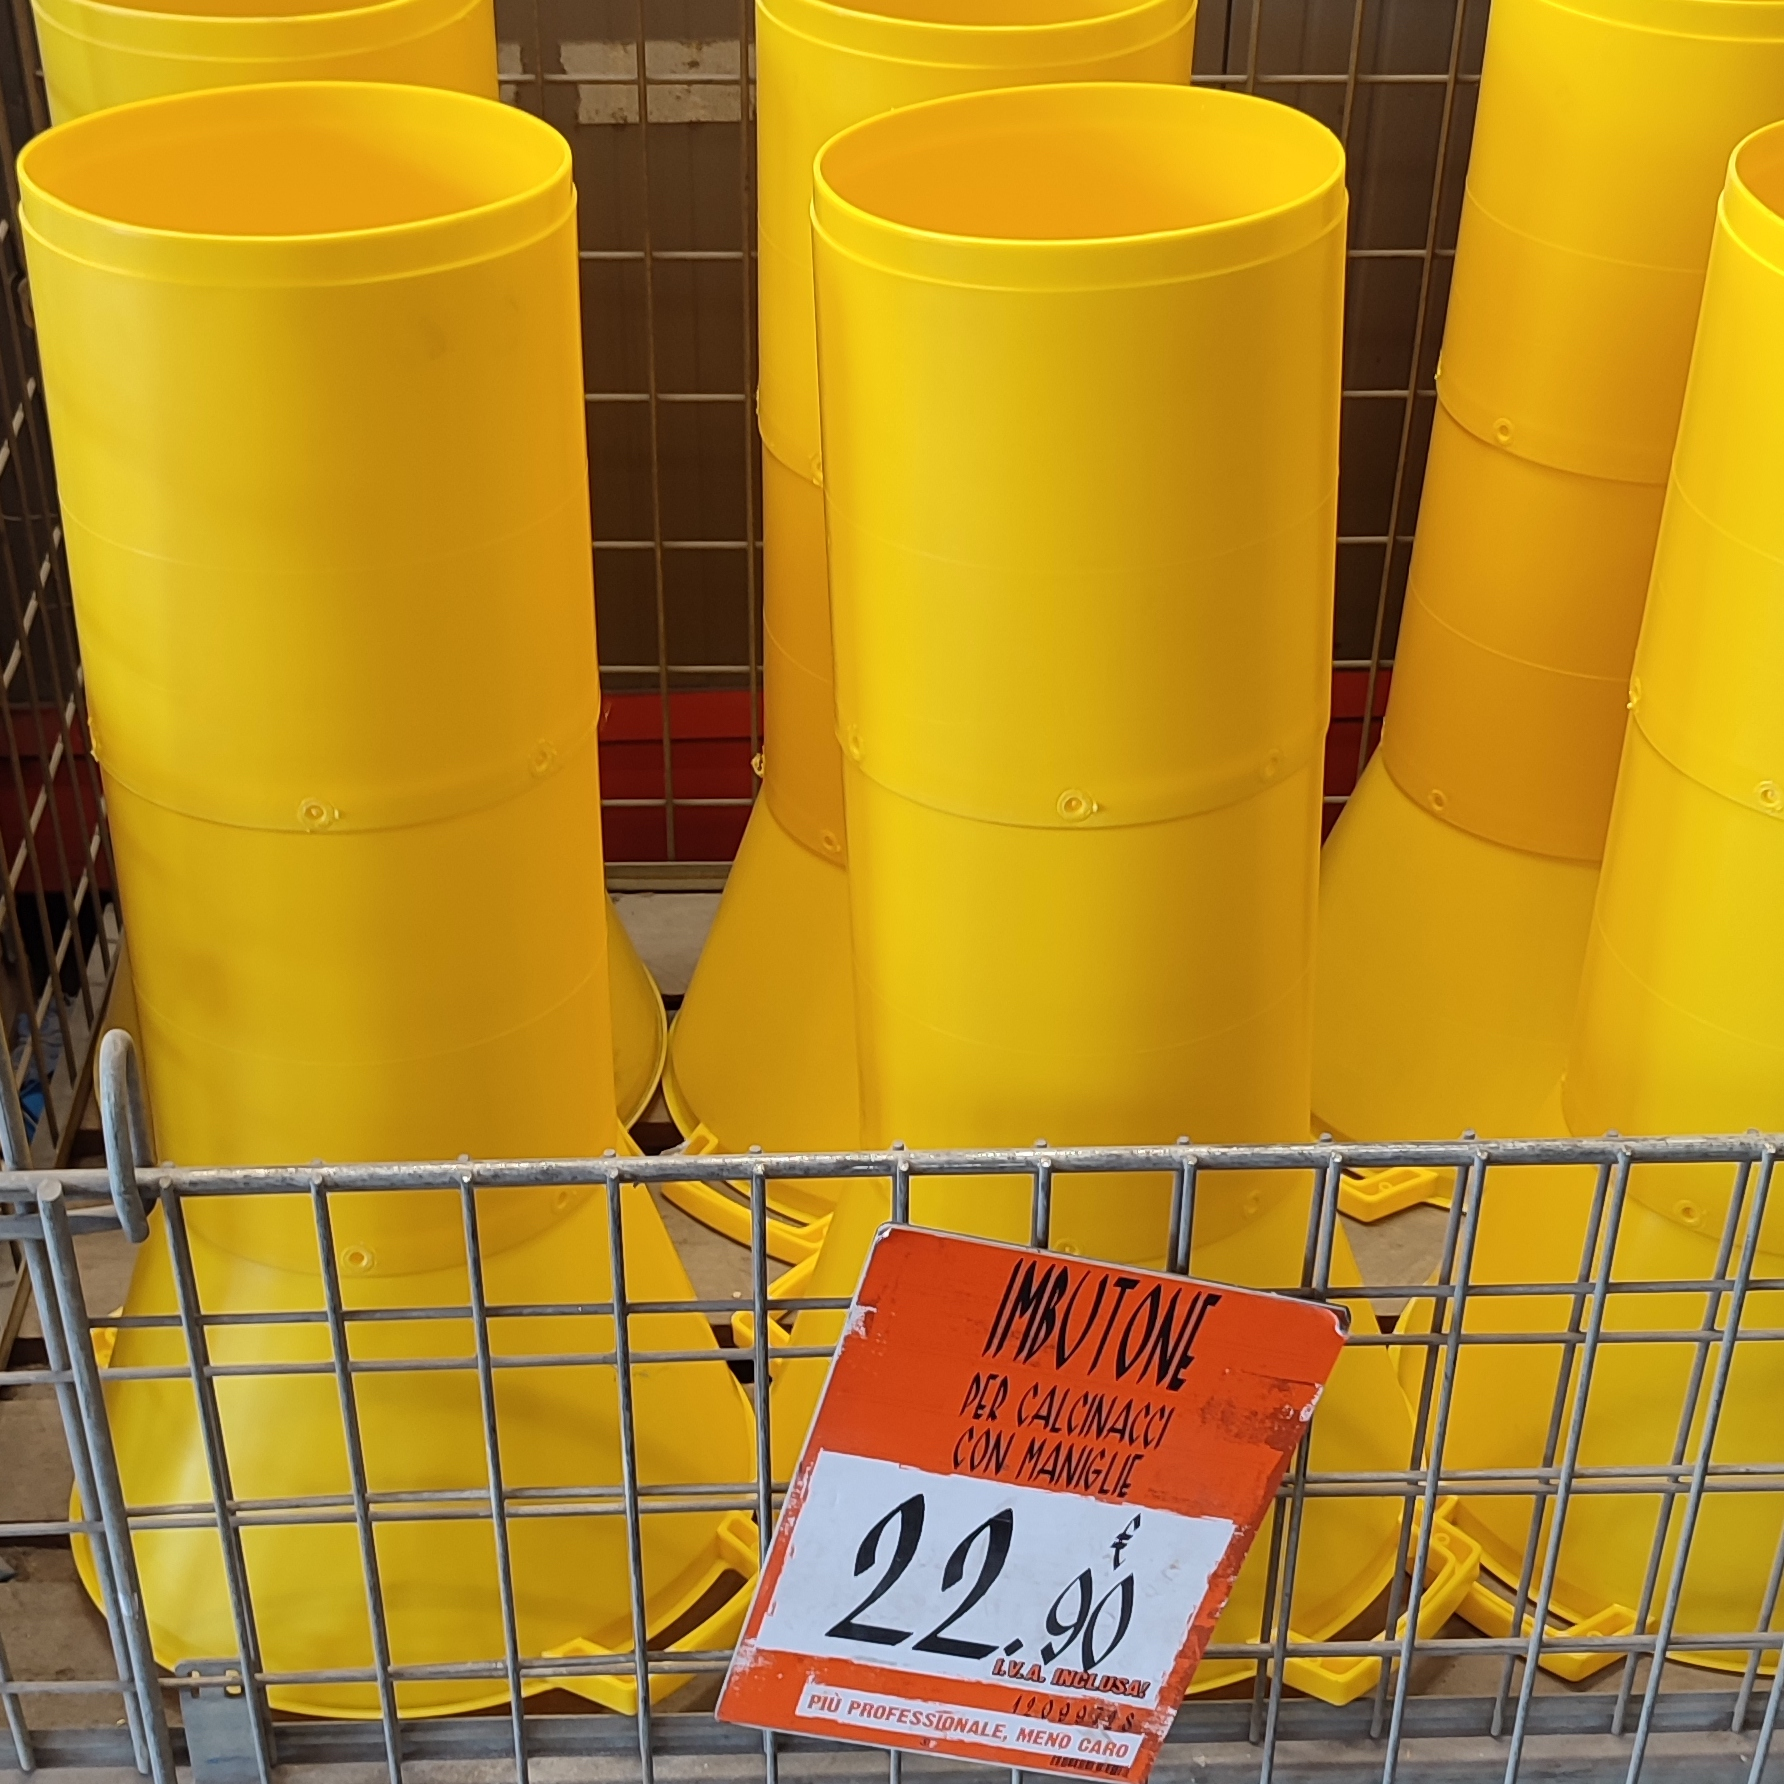
\includegraphics[width=.45\columnwidth]{Graphics/foto/1697454976316}} \quad
\subfloat[]
{
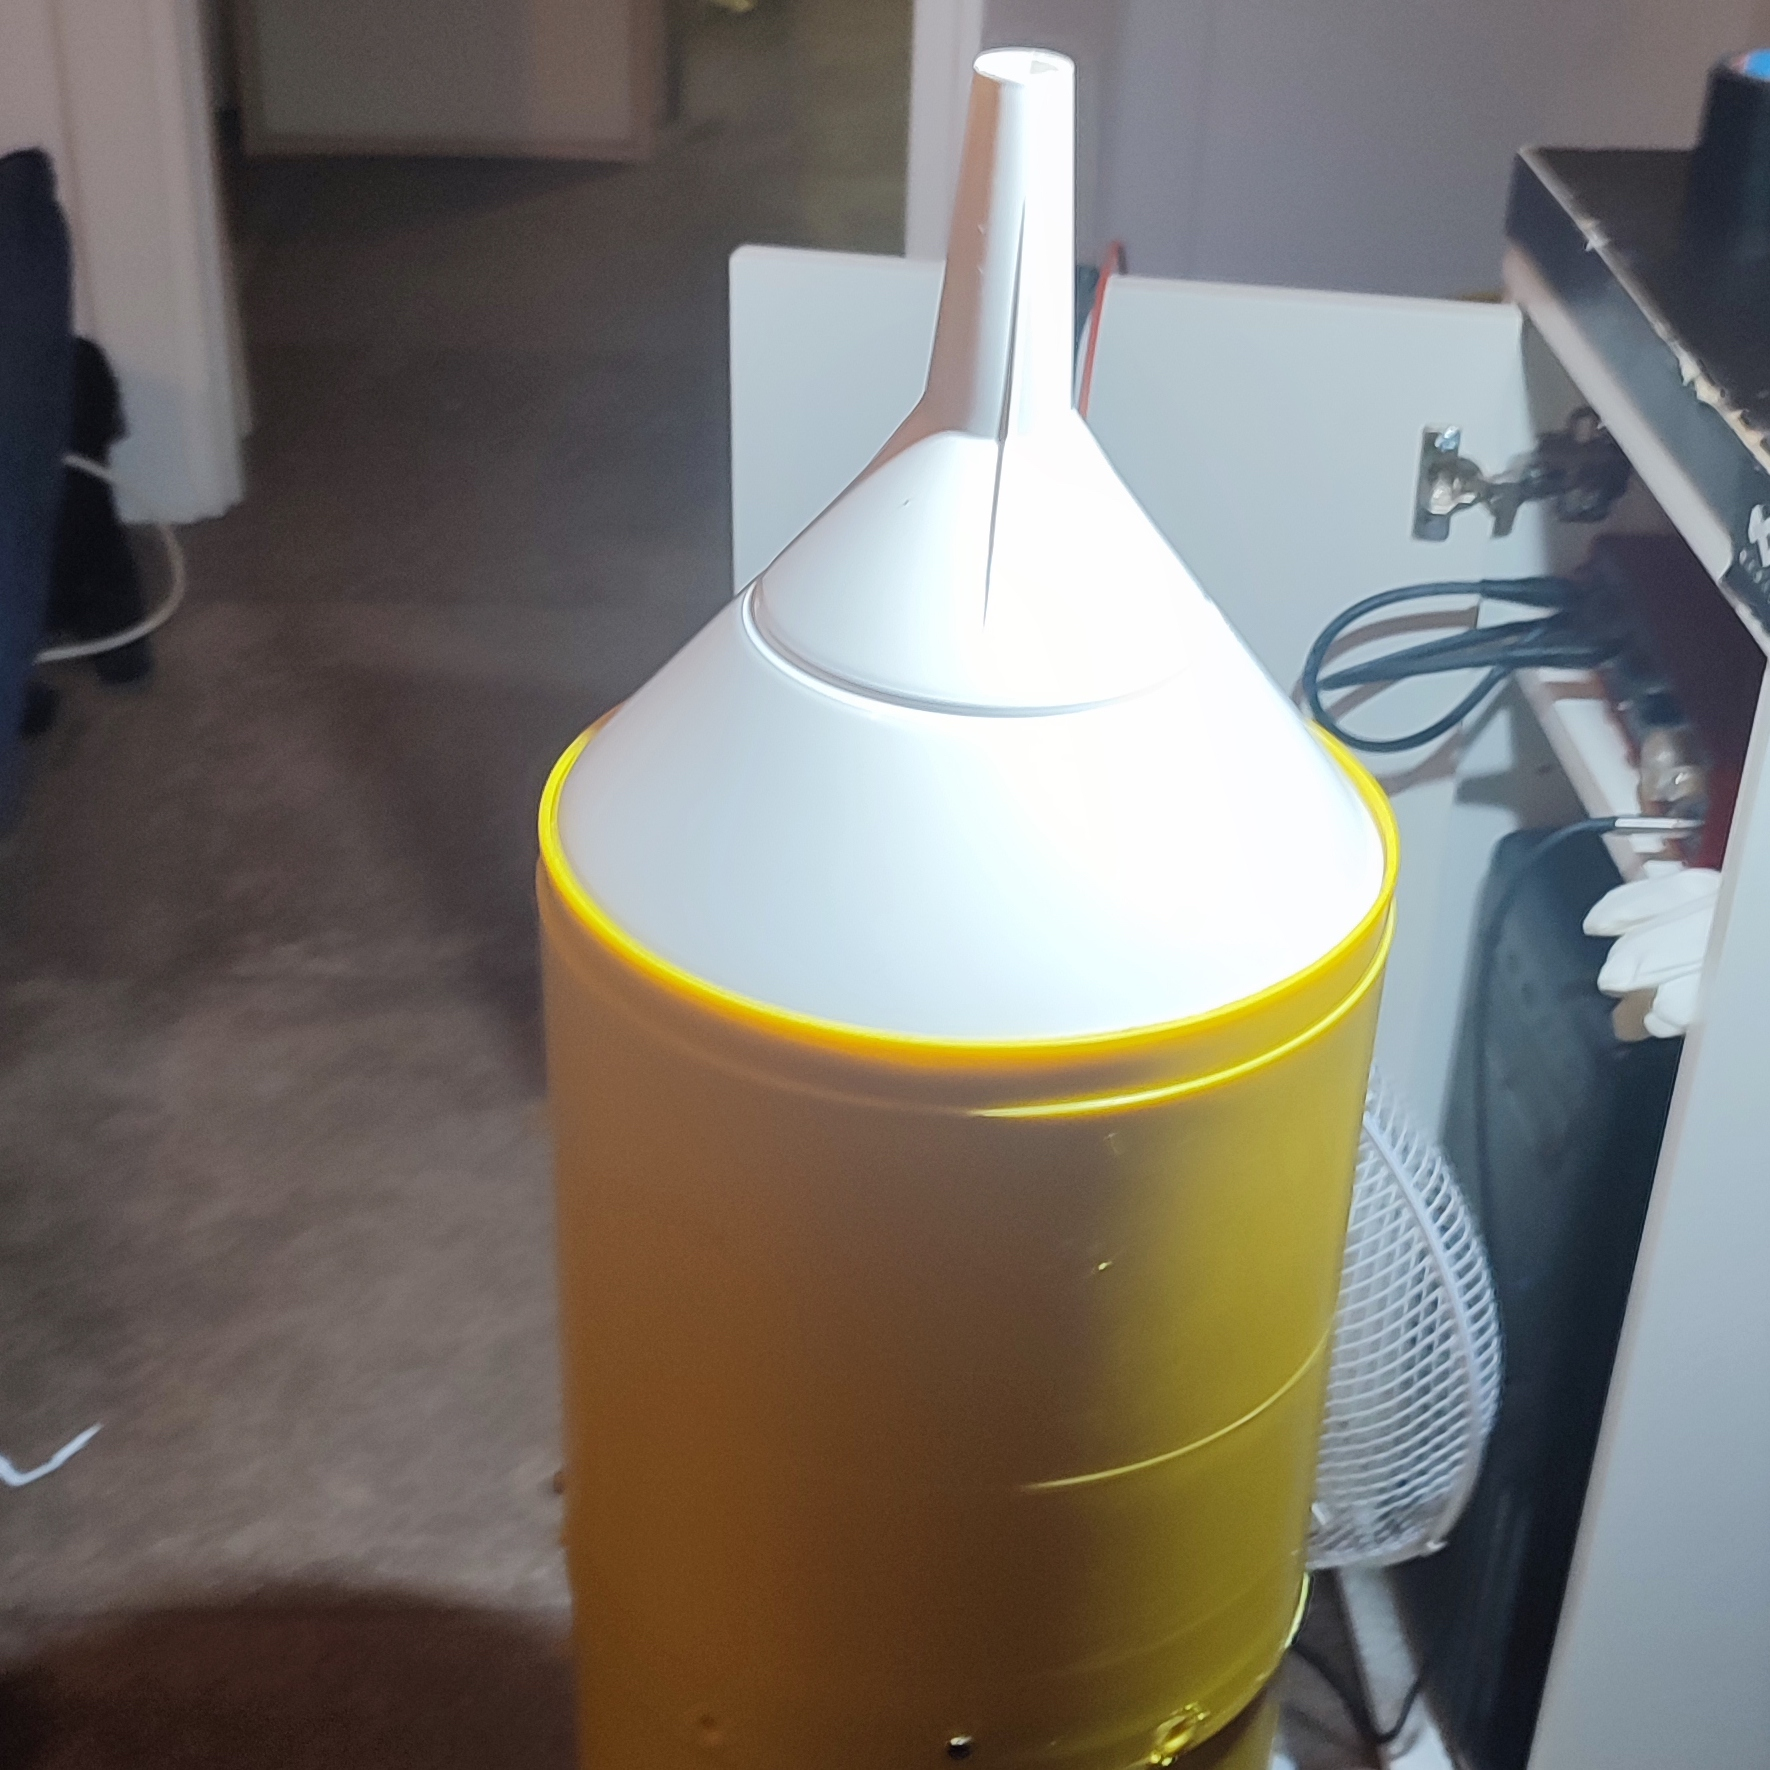
\includegraphics[width=.45\columnwidth]{Graphics/foto/1697454976170}} \\
\subfloat[]
{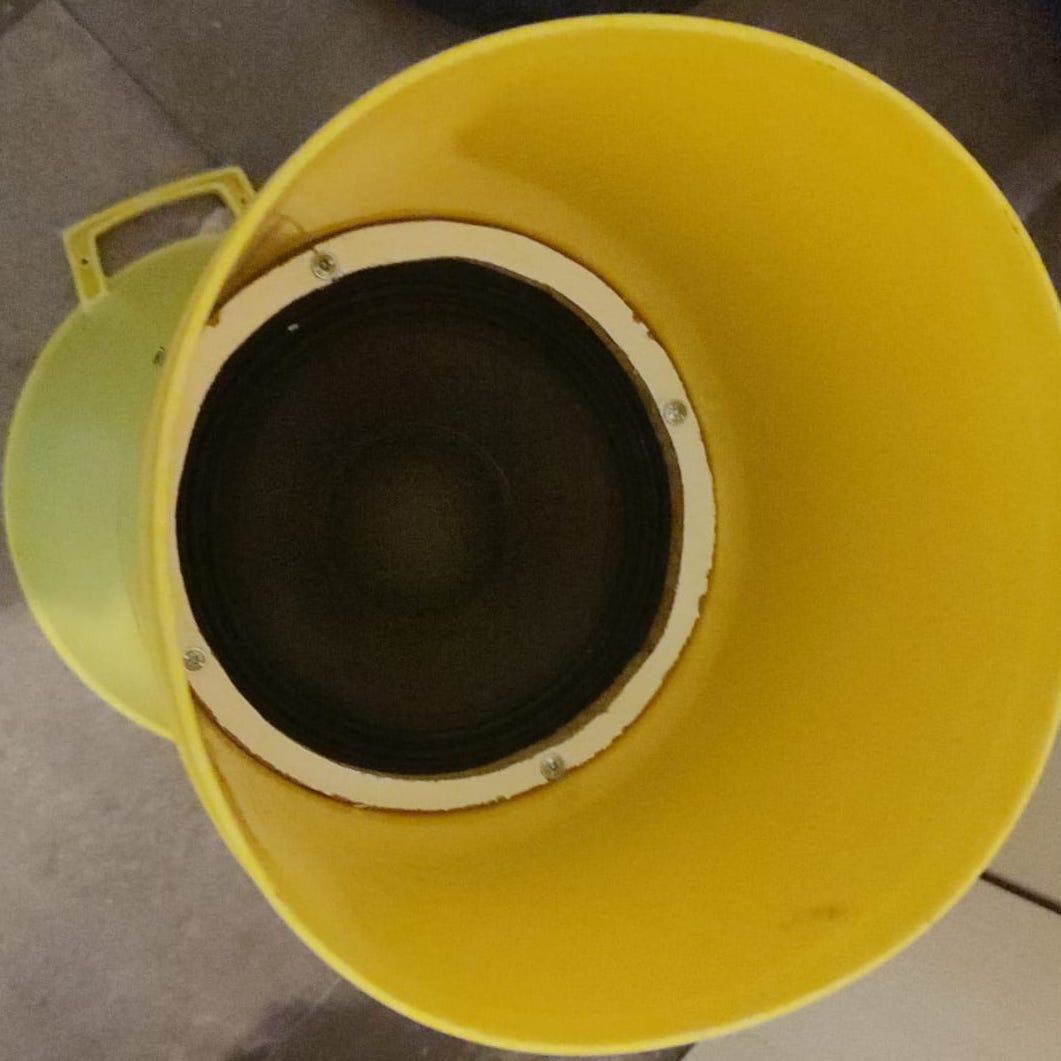
\includegraphics[width=.45\columnwidth]{Graphics/foto/IMG-20230925-WA0002}} \quad
\subfloat[]
{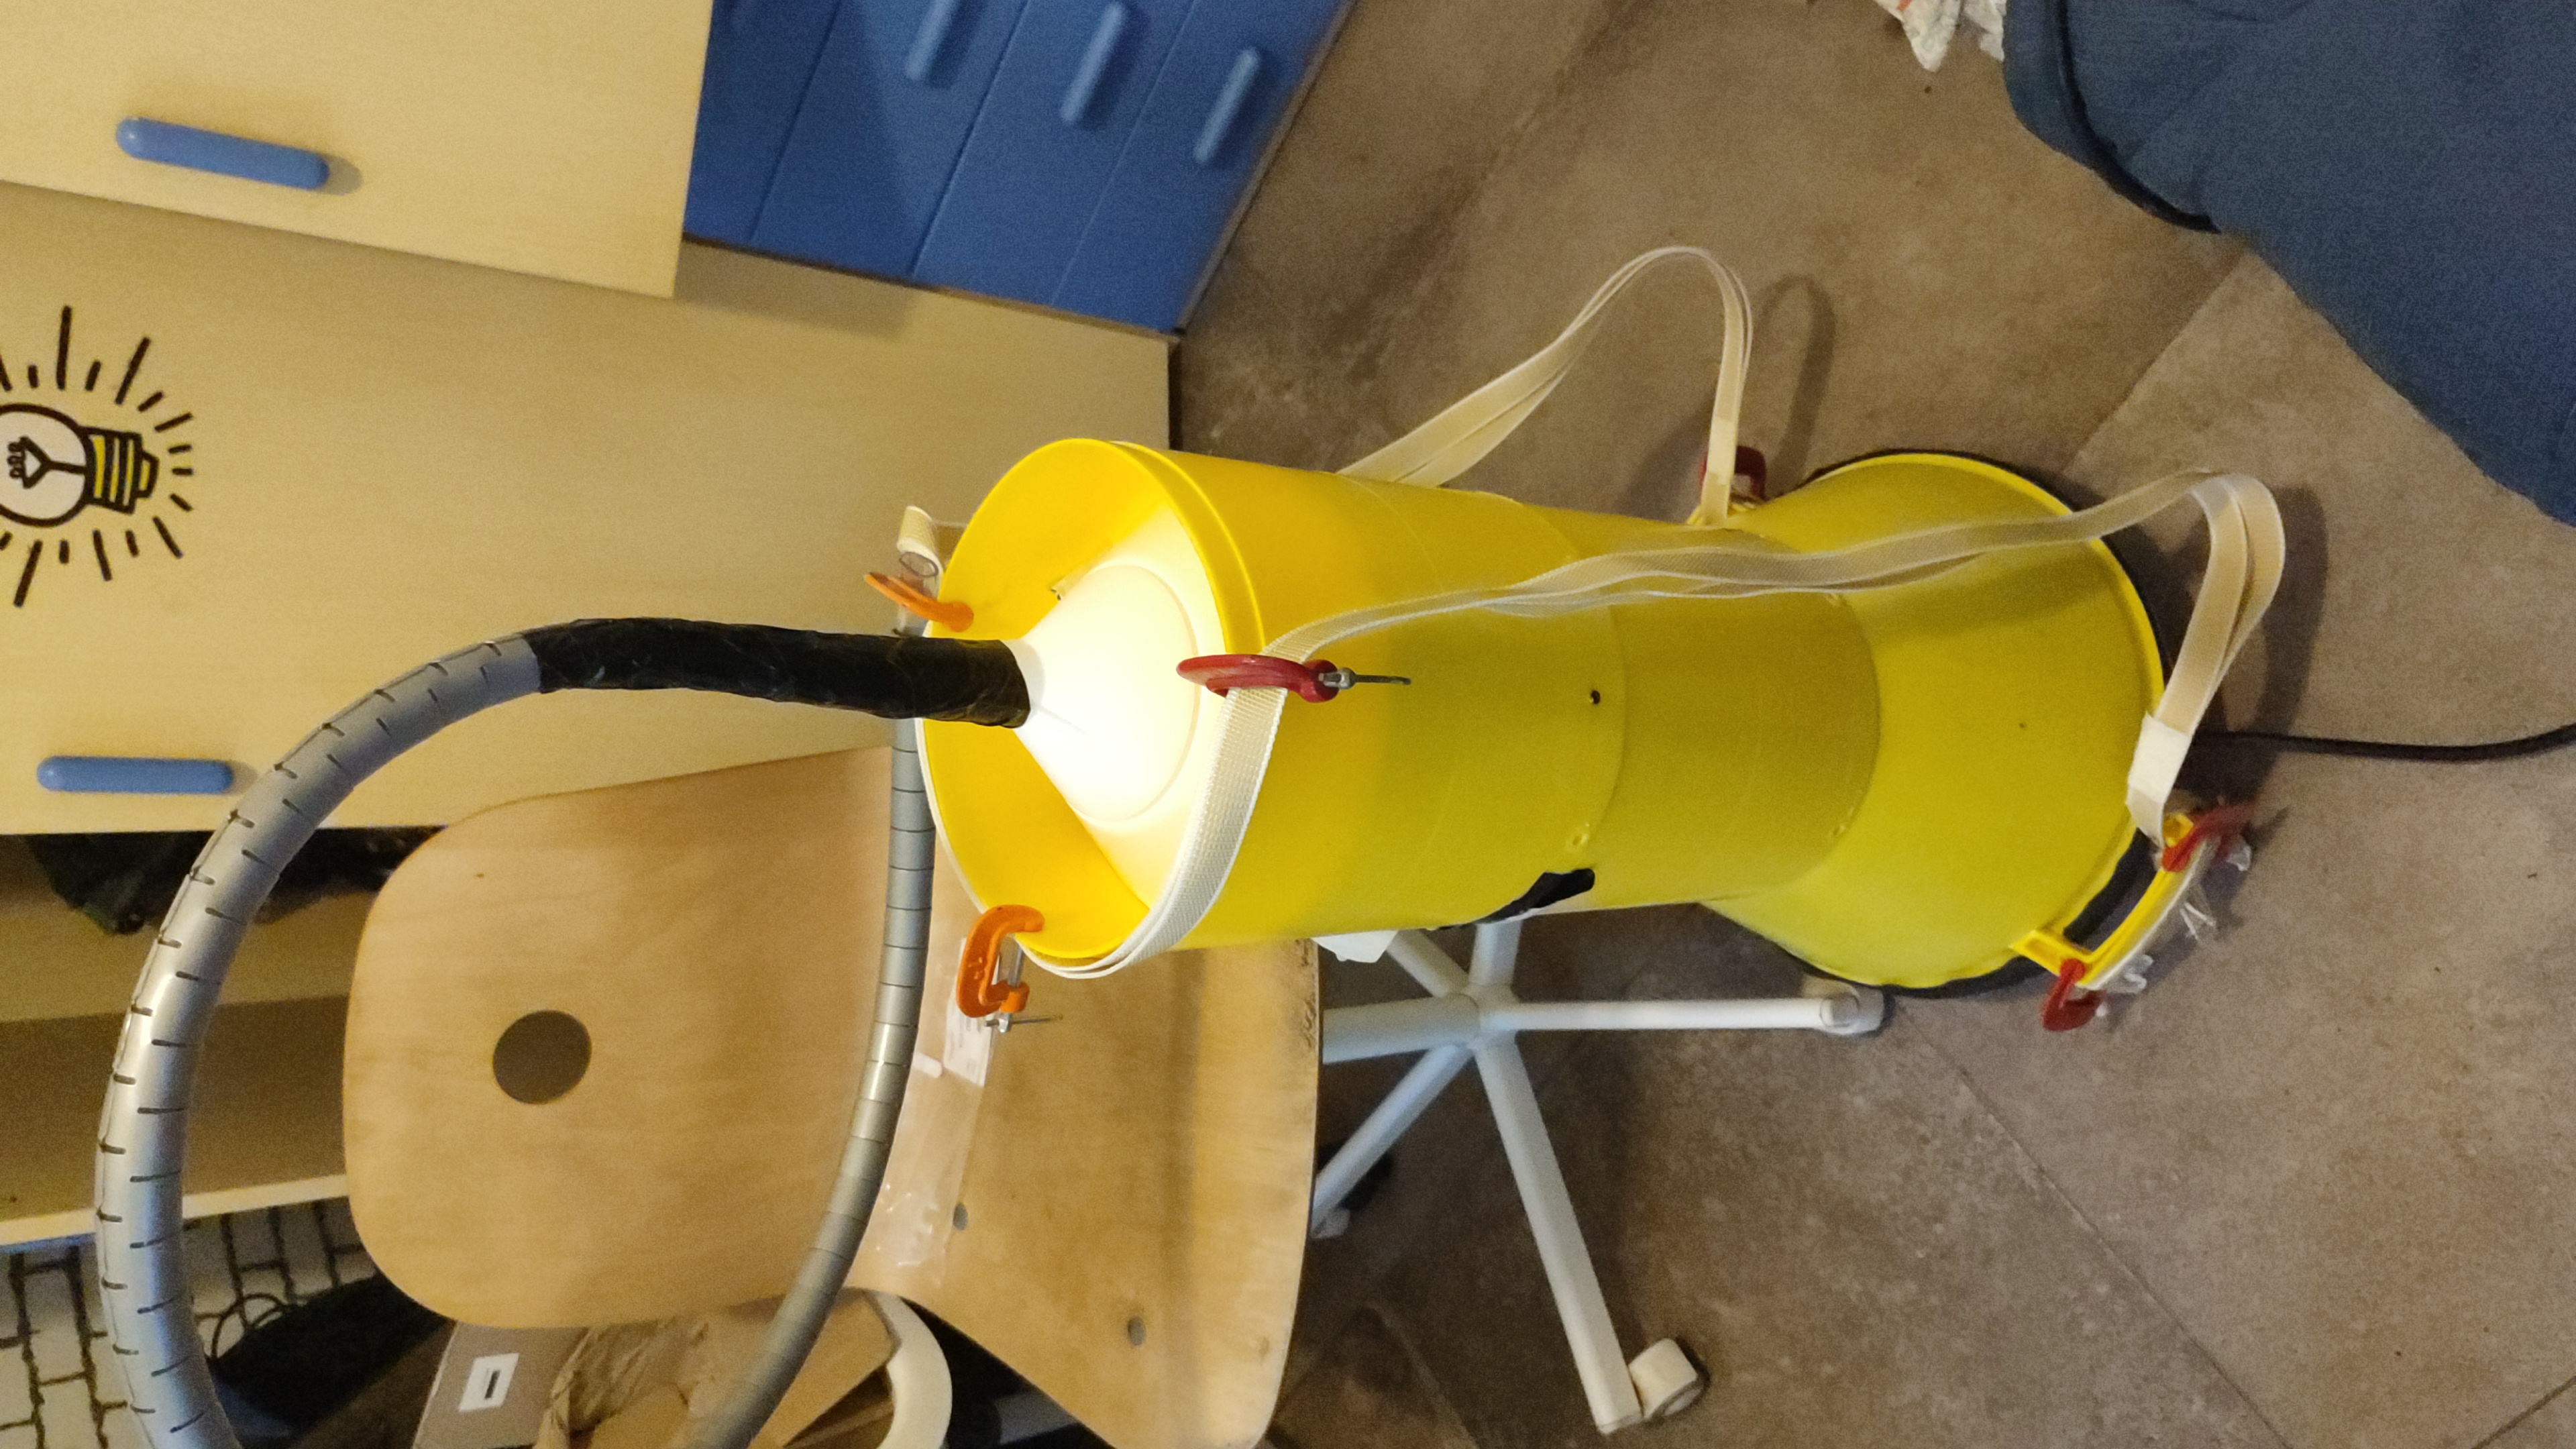
\includegraphics[width=.45\columnwidth]{Graphics/foto/1697478266898}}
\caption{Imbutone}
\label{fig:imbutone}
\end{figure}

È stato possibile trovare in commercio un imbuto di plastica con un diametro nominale di 22cm che riesce ad incastrarsi perfettamente all’interno del cilindro dell’imbutone [Fig. \ref{fig:imbutone}].

Per inserire l’altoparlante all’interno del cilindro dell’ imbutone è stato realizzato un anello in legno [Fig. \ref{fig:imbutone}].

L’anello è stato fissato alla struttura tramite quattro viti di legno. In tal modo è stato possibile inserire l’altoparlante nel cilindro poggiandolo sull’anello di legno e fissando anche esso con delle viti [Fig. \ref{fig:imbutone}]. Per non correre il rischio di fuoriuscite di pressione del flusso dalla parte dell’altoparlante, l’anello di legno è stato sigillato con del silicone da ambedue le parti.

La posizione dell’altoparlante è stata scelta tramite una serie di prove di suono empiriche con lo scopo di trovare la migliore risonanza.

È stato necessario insonorizzare internamente tutta la parte inferiore dell’imbutone. A tal proposito è stato realizzato un coperchio in legno corrispondente esattamente al disegno della faccia posteriore dell’imbutone, manici compresi [Fig. \ref{fig:imbutone}].

Sia la parete interna della parte bassa dell’imbutone, che la facciata interna del coperchio di legno sono state rivestite con una spugna insonorizzante ondulata [Fig. \ref{fig:imbutone}].

Per far ciò è stato necessario disegnare geometricamente lo sviluppo del tronco di cono, equivalente a un arco di corona circolare e ritagliarlo sulla spugna insonorizzante [Fig. \ref{fig:imbutone}]. È stato più agevole insonorizzare la parte di cilindro intermedia tra l’altoparlante e il tronco di cono, in quanto essa corrispondeva a un rettangolo di cui era facile calcolare la base e l’altezza.

Per far aderire il tappo di legno all’imbutone sono stati applicati alle maniglie quattro morsetti.
Un tubo di gomma, incastrandosi da entrambi gli estremi, collega la parte terminale dell’imbuto di diametro $22 cm$ con il flauto. Il collegamento del tubo con l’imbuto è stato rinforzato con del nastro telato. Il tubo di plastica essendo soggetto a piegamenti è stato rivestito con una canalina passa cavi per mantenere una forma curvilinea.

La pressione generata dal sistema ha consentito di reinserire il tappo all’interno della testata  rimuovendo l’asta filettata  in modo da lasciare libero un foro per il passaggio dell’aria. La presenza del tappo ha consentito di poter mantenere pressoché inalterato  il rapporto tra le ottave.

Infine delle cinte da serranda sono state applicate a tutta la struttura in modo tale da formare due bretelle che consentono all’interprete di avere stabilmente il prototipo sulle spalle. [Fig. \ref{fig:imbutone}]

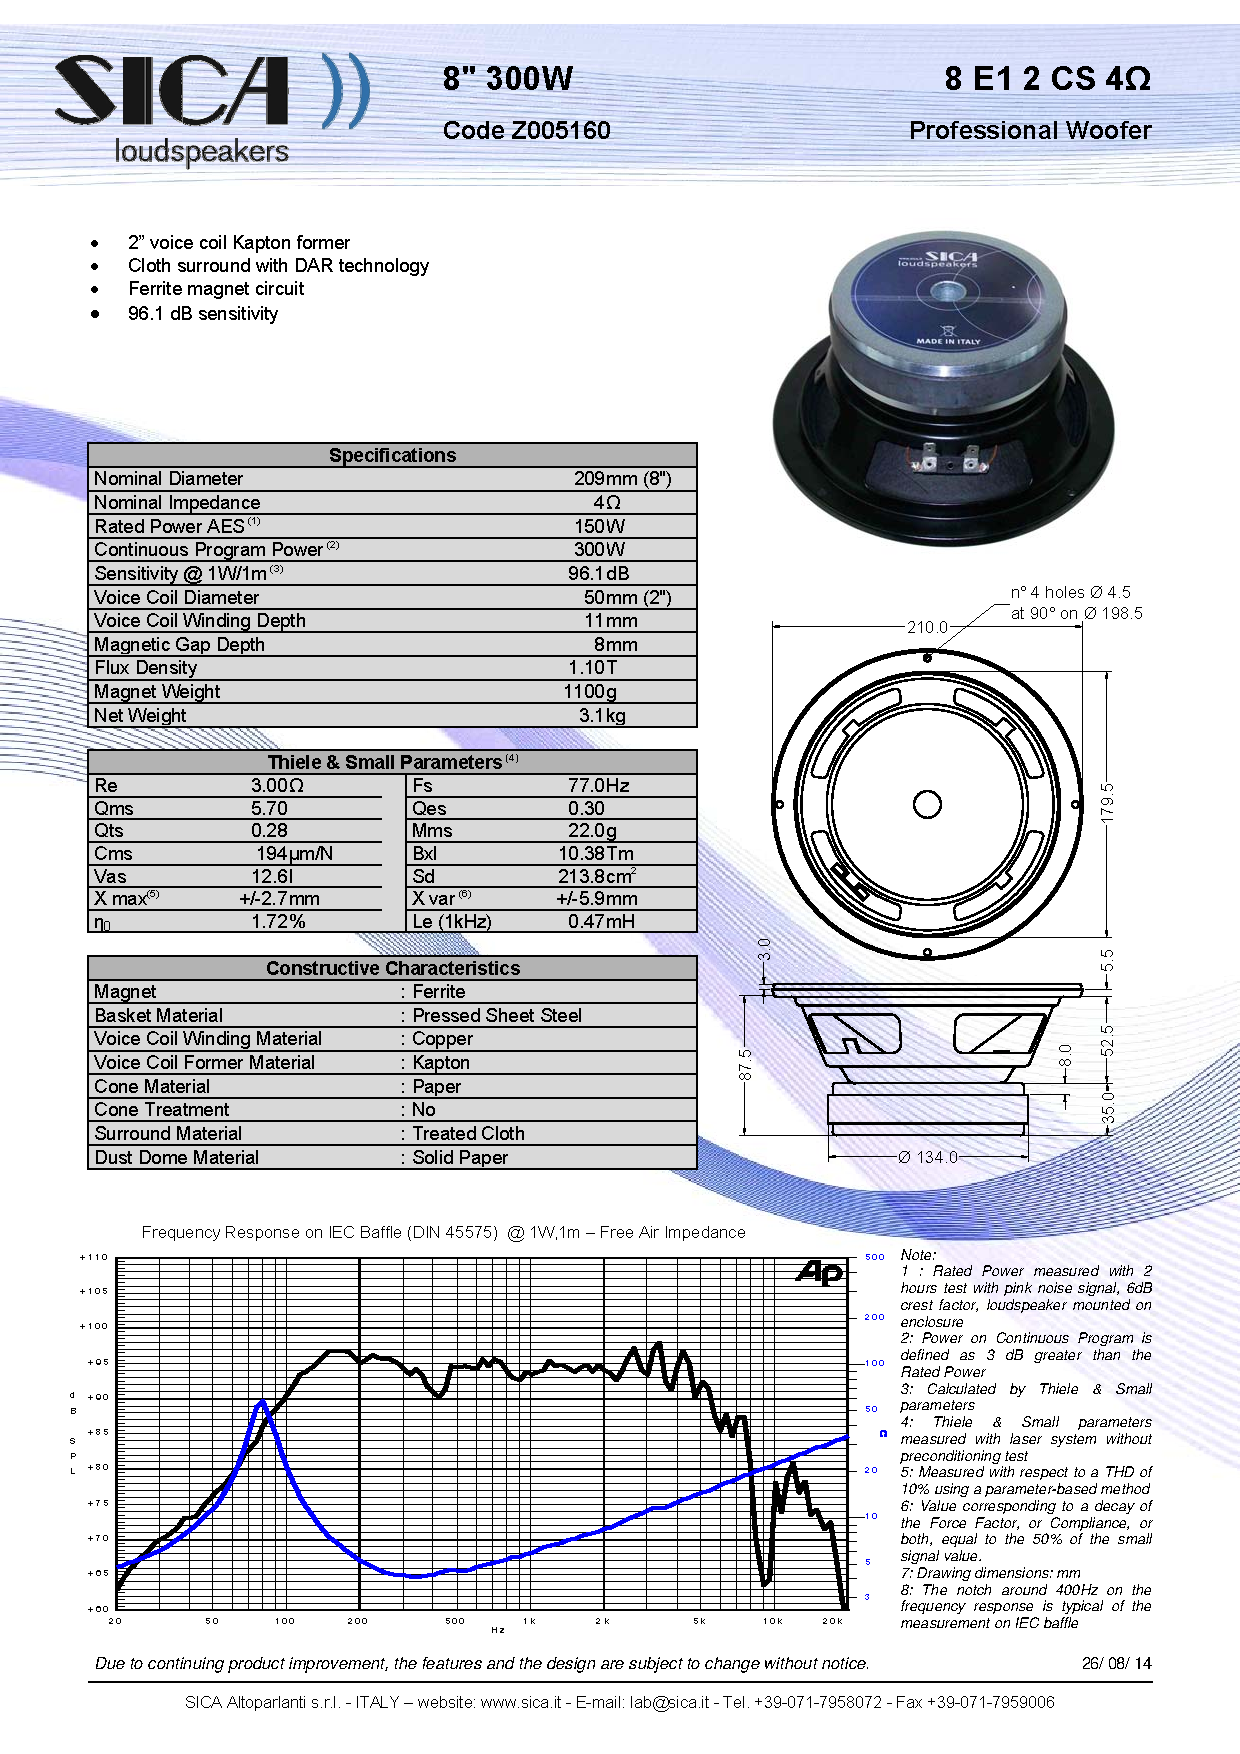
\includepdf[pages=-]{Graphics/foto/Z005160C.pdf}

% !TEX TS-program = pdflatex
% !TEX root = ../tesi.tex

%************************************************
\chapter{LA RICERCA MUSICALE}
\label{chp:ricerca}
%************************************************

Una volta messo a punto  lo strumento sono iniziati i processi di ricerca  per capirne le potenzialità musicali.

Già durante il processo di  sviluppo del sistema altoparlante-flauto, anche se appena accennate,  sono affiorate alcune potenzialità sonore molto interessanti:
Usando  basse frequenze si formano frullati o tremoli, delicati e controllati, non realizzabili con un flauto tradizionale
 Nella banda critica si accentuano i battimenti dal momento che il suono entra direttamente dentro lo strumento.
Queste potenzialità sono state approfondite con lo strumento ultimato, specificando quattro modalità operative:
Con l’uso di una sinusoide pura tra i 1hz e i 100 hz si ricava un tremolo controllato dentro il flauto. Le diverse  frequenze del tremolo variano  in base alla frequenza della sinusoide,
Alla frequenza della sinusoide del punto 1 si somma  una altra sinusoide, anche essa tra i 1 hz e i 100 hz , formando così una modulazione di frequenza.  Con questa modalità risulta possibile sviluppare spettri più ricchi creano leggere variazioni ritmiche  nel tremolo .
Con l’uso di un rumore bianco, filtrato con un bandpass di trentaduesimo ordine, e  con un q variabile ma  molto stretto,si ricava, con frequenze molto gravi, un leggero senso di indeterminabilità . Viene così prodotta  una ritmicità che pur controllata ha una tendenza verso l’aleatorietà.          Quando questa modalità viene  spostata  nelle

bassissime frequenze aggiunge alle precedenti sonorità simili a soffi date dallo spingere i filtri al limite della rottura.
Per quanto riguarda la zona della  banda critica, una modulazione ad anello del suono del flauto catturato con un microfono, moltiplicato   con una sinusoide tra i 20hz e i 50 hz, produce  dei battimenti su ogni formante del flauto creando spettri ricchissimi.

Il brano, ancora in fase di sviluppo, in alcune zone, denominate “voci” necessita dell’ascolto vicendevole e della simultanea collaborazione  dei due interpreti, il flautista ed il live electronics, per la ricerca della massima sintonia possibile in presenza di continue variazioni determinate da scelte alternate dei due interpreti.
Ognuna di queste scelte è determinata da tre possibilità, espresse in partitura,  che l’interprete è libero di optare. L’altro interprete, ascoltata e capita la scelta, agisce conseguentemente alle indicazioni in partitura relative alla scelta operata dal primo.
Le “voci” sono un “tempo sospeso”, non riportato in partitura e non determinabile a priori.

Per quanto riguarda l’elettronica  in partitura sono indicate le modalità di operazione:
Sine = sinusoide
FM = modulazione di frequenza


N = noise
RM  = modulazone di ampiezza
Di seguito a queste modalità di operazione è indicato il range frequenziale nel quale operare.
Per quanto riguarda la modulazione di frequenza il primo range riguarda la modulante e il secondo della portante.
Nel noise il primo parametro indica la frequenza di operazione e il secondo il q.
I vari gesti di l.e. sono completati con delle indicazioni grafiche che descrivono prima i percorsi frequenziali e poi gli andamenti dinamici dei percorsi di ampiezza.
Ogni “voce” ha al suo interno tre possibilità di scelta di gesto sonoro.
Il verso di una freccia indica quale è l’ interprete  che deve operare la scelta.
La scelta operata produce una modalità sonora che deve essere riconosciuta dall’altro interprete in modo da potersi sintonizzare con essa.
In questo “tempo sospeso” nessuno dei due interpreti smette di suonare  in quanto il primo continua nella sua modalità ed il secondo sperimenta la sincronizzazione.
Non esistono  dei tempi definiti per la  durata di ogni “voce”.
Infatti l’istante di ritorno alla partitura non risulta prevedibile  in quanto  sarà in completa gestione dell’interprete “comandante” nella “voce”suonata.

In questo modo si formano due interpreti bicamerali.
L’interprete comandante diventa in questo modo parte emotiva e “allucinazione sonora” del secondo interprete. Infatti il secondo interprete riceve l’ordine del gesto sonoro dal primo e tramite ascolto e processi logici deve eseguire  il conseguente gesto sonoro.

\input{capitoli/05-conclusioni}
% !TEX TS-program = pdflatex
% !TEX root = ../tesi.tex

%************************************************
\chapter*{RINGRAZIAMENTI}
%************************************************

Vorrei fare i dovuti ringraziamenti alle persone che mi hanno accompagnato in questo percorso.

Ringrazio la mia famiglia: mio padre Mauro e mia madre Rita, per avermi dato per avermi totalmente supportato con affetto e amore, e anche non meno importante per aver sopportato la follia che ho portato negli ultimi mesi.

I miei amici di sempre: Eugenio Federico Daniele, per esserci sempre stati e  per tutte le serate insieme.

A l’altro amico di sempre Federico.
Agli amici del mare che ogni estate, purtroppo non questa, mi hanno regalato momenti indimenticabili.

Al mio compagno di studio Giulio per questi quattro anni passati insieme.
Ad Alessandro per essersi offerto per suonare questo strumento.

Ad Andrea, il mio insegnante di chitarra, per aver dato il via alla mia passione musicale con il mio primo approccio ad uno strumento.

Ai maestri di composizione  Nicola Bernardini e Pasquale Citera per avermi affiancato questo viaggio attraverso la musica.

Alla maestra Silvia Lanzalone che in questo viaggio  mi accompagnerà in futuro.

Infine, non per importanza anzi, al maestro Giuseppe Silvi per avermi accompagnato e supportato in questi mesi di follia e creatività e con una grande passione e devozione alla causa incredibile con lui voglio ringraziare anche gli altri membri del LEAP per avermi accolto in questo spazio stupendo in cui si respira musica e ricerca in ogni angolo, grazie in oltre per averlo costruito anche mediamente vicino a casa mia

